%%%%%%%%%%%%%%%%%%%%%%%%%%%%%%%%%%%%%%%%%%%%%%%%%%
%%%%%%%%%%%%%%%%% Documentclass %%%%%%%%%%%%%%%%%%
%%%%%%%%%%%%%%%%%%%%%%%%%%%%%%%%%%%%%%%%%%%%%%%%%%
\documentclass[fontsize=12pt,		% Font size
			   toc=listof,			% List of... into table of contents % listofnumbered
			   paper=A4,			% A4 paper
			   headinclude=true,	% Include header into type area calculation
			   footinclude=false,	% Don't include footer into type area calculation
			   headsepline=true,	% Separating line between header and text
			   footsepline=false,	% Separating line between footer and text
			   DIV=calc,			% Auomatically calculate DIV
			   %BCOR=15mm,			% Binding correction
			  ]{scrbook}

%%%%%%%%%%%%%%%%%%%%%%%%%%%%%%%%%%%%%%%%%%%%%%%%%%
%%%%%%%%%%%%%%%%%%%% Packages %%%%%%%%%%%%%%%%%%%%
%%%%%%%%%%%%%%%%%%%%%%%%%%%%%%%%%%%%%%%%%%%%%%%%%%

% Encoding, fonts, etc...
\usepackage[english]{babel}	% Language package
\usepackage[utf8]{inputenc}			% Files are UTF-8 encoded
\usepackage[T1]{fontenc}			% Font encoding
\usepackage{lmodern}				% Scalable font
\usepackage{microtype}				% Nicer typesetting
\usepackage{relsize}				% Relative font size (for macros)
\usepackage{setspace}				% Spacehandling

% Math
\usepackage{amsmath}
\usepackage{amsfonts}
\usepackage{amssymb}
\usepackage{textcomp}				% Avoids conflicts between siunitx and microtype
\usepackage{siunitx}				% Allow for german decimals, e.g. 1,344 instead of 1.344 + other stuff
\usepackage{nicefrac}				% Schräggestellte Brüche...

% Include MATLAB code (see http://www.howtotex.com/tips-tricks/how-to-include-matlab-code-in-latex-documents/)
% the file mcode.sty must be placed in the same folder as main.tex 
% add options between square brackets: bw for b/w printing, numbered for numbered lines, framed for framing the code,
\usepackage[framed,numbered,autolinebreaks,useliterate]{mcode}	

% Package and options for nice inspirational quotes - takes one argument - the author of the quote.
\makeatletter
%\renewcommand{\@chapapp}{}% Not necessary...
\newenvironment{chapquote}[2][2em]
  {\setlength{\@tempdima}{#1}%
   \def\chapquote@author{#2}%
   \parshape 1 \@tempdima \dimexpr\textwidth-2\@tempdima\relax%
   \itshape}
  {\par\normalfont\hfill--\ \chapquote@author\hspace*{\@tempdima}\par\bigskip}
\makeatother			

% Graphics, figures, tables...
\usepackage{graphicx}				% Allow graphics
\usepackage{xcolor}					% Allow colors
\usepackage{booktabs}				% Nicer tables
\usepackage{multirow} 				% Make multiple rows one big row in a table
%\usepackage{longtable}
\usepackage{tikz} 					% For generation of vector graphics
\usepackage{pgfplots}				% For nice plots
\usepackage{listings}				% Source code listings
\usepackage[plain,					% Float wrapper for algorithms
			chapter]{algorithm}
\usepackage{algorithmic}			% Pseudo-code for algorithms
%\usepackage{changepage} 			% Margin adjustments for big figures
%\usepackage{rotating} 				% Rotate figures if needed
%\usepackage{lscape}					% Landscape pages
\usepackage{subcaption}				% Figures with multiple images, (a), (b) ...
\usepackage{pdfpages}				% Inserting of full pages from pdf files
\usepackage{framed}					% All kinds of framed stuff
\usepackage{placeins}				% Lets you use barriers for figures
%\usepackage{varioref}				% Stellt den Befehl \vref{} zur Verfügung --> für Hinweis auf Ziel des Verweises

% Nice titlepage with more fields for scientific writeups
%\usepackage{titlepage}

% Glossary & index
%\usepackage{glossaries}			% Can be used to create a nice glossary
\usepackage{makeidx}				% Can be used to create a sorted index

% Bibliography, citations...
\usepackage{xkeyval}

\usepackage[backend=biber,
			bibstyle=alphabetic,
			citestyle=alphabetic,
			maxbibnames=4,
%			%firstinits=true,
			giveninits=true,
			hyperref=true,
			backref=true]{biblatex}
%\usepackage{biblatex}			
\usepackage{url}
\usepackage[autostyle=tryonce]{csquotes}
\usepackage[plainpages=false]{hyperref}
%\usepackage[all]{hypcap}

% other
\usepackage{ifthen}					% Allows conditional statements
\usepackage{blindtext}				% Blindtext for testing purposes
\usepackage{scrhack}				% Hacks that allow a better integration of non-koma-scripts with komascript

%%%%%%%%%%%%%%%%%%%%%%%%%%%%%%%%%%%%%%%%%%%%%%%%%%
%%%%%%%%%%%%%%%%%%%%% Config %%%%%%%%%%%%%%%%%%%%%
%%%%%%%%%%%%%%%%%%%%%%%%%%%%%%%%%%%%%%%%%%%%%%%%%%

% babel
\selectlanguage{english}

%%%%%%%%%%%%%%%%%%% spacing %%%%%%%%%%%%%%%%%%%%%
\onehalfspacing
%%%%%%%%%%%%%%%%%%% /spacing %%%%%%%%%%%%%%%%%%%%%

% biblatex
\addbibresource{bibliography.bib}	% Add bibliography file
%\DefineBibliographyStrings{ngerman}	% et al. instead of u.a.
%	{andothers=
%	{et\addabbrvspace al\adddot}}

% titlepage
%\TitlePageStyle[]{KOMAScript}

% TikZ
%\usetikzlibrary{shapes}			% Shapes for Tikz
\usetikzlibrary{plotmarks}			% Plot marks for Tikz
\usetikzlibrary{calc}				% For general calculations
\usetikzlibrary{intersections}		% Can calculate intersections in tikz
\usetikzlibrary{patterns}			% For bar plots etc.
\usetikzlibrary{arrows}				% For arrow heads
\usetikzlibrary{arrows.meta}		% ... seems like I need this as well?
\newlength\figureheight 			% Variables for figures exported with matlab2tikz
\newlength\figurewidth
\newcommand\figurescale{1}

% pgfPlots
\pgfplotsset{compat=newest} 
\pgfplotsset{plot coordinates/math parser=false}
\pgfkeys{/pgf/number format/.cd ,use comma ,set thousands separator={ }}
% The following is a hack to make pgfplots load files from directories other than the current one
\makeatletter
\def\pgfplotstableread@openfile{%
    \def\pgfplotstable@loc@TMPa{\pgfutil@in@{ }}%
    \expandafter\pgfplotstable@loc@TMPa\expandafter{\pgfplotstableread@filename}%
    \ifpgfutil@in@
        \t@pgfplots@toka=\expandafter{\pgfplotstableread@filename}%
        \edef\pgfplotstableread@filename{\pgfplots@dquote\the\t@pgfplots@toka\pgfplots@dquote}%
    \fi
    \let\pgfplotstableread@old@crcr=\\%
    \def\\{\string\\}% just to make sure we don't try to open inline table data...
    \openin\r@pgfplots@reada=\csname pgfk@/pgfplots/table file path\endcsname\pgfplotstableread@filename.tex
    \ifeof\r@pgfplots@reada
        \openin\r@pgfplots@reada=\csname pgfk@/pgfplots/table file path\endcsname\pgfplotstableread@filename\relax
    \else
        \pgfplots@warning{%
            You requested to open table '\pgfplotstableread@filename', but there is also a '\pgfplotstableread@filename.tex'. 
            TeX will automatically append the suffix '.tex', so I will now open '\pgfplotstableread@filename.tex'.
            Please make sure you don't accidentally load TeX files - this may produce unrecoverable errors.}%
        \closein\r@pgfplots@reada
        \openin\r@pgfplots@reada=\pgfplotstableread@filename\relax
    \fi
    %
    \ifeof\r@pgfplots@reada
        \pgfplotsthrow{no such table file}{\pgfplots@loc@TMPa}{\pgfplotstableread@filename}{Could not read table file '\csname pgfk@/pgfplots/table file path\endcsname\pgfplotstableread@filename'. In case you intended to provide inline data: maybe TeX screwed up your end-of-lines? Try `row sep=crcr' and terminate your lines with `\string\\' (refer to the pgfplotstable manual for details)}\pgfeov%
        \global\let\pgfplotstable@colnames@glob=\pgfplots@loc@TMPa
        \def\pgfplotstableread@ready{0}%
    \fi
    \pgfplots@logfileopen{\pgfplotstableread@filename}%
    \let\\=\pgfplotstableread@old@crcr
}
\makeatother
\pgfplotsset{table file path/.initial = {./}}

% siunitx
\sisetup{locale = US}

% listings
\lstset{ %
backgroundcolor=\color{white}, % background color
basicstyle=\footnotesize\ttfamily,% code font size
breakatwhitespace=false, % automatic breaklines only at whitspaces?
breaklines=true, % automatic breaklines
captionpos=b, % caption position
%commentstyle=\color{green}, % comment style
deletekeywords={}, % delete keywords from language
escapeinside={(*@}{@*)}, % LaTeX will be evaluated inside (*@ \code{} @*)
extendedchars=true, % Non-ASCII characters
frame=single, % frame around code
keepspaces=true, % keep spaces (i.e. indentation), might need columns = flexible
%columns=flexible, % set characters in columns or freely?
%keywordstyle=\color{blue}, % keyword style
language=C++, % programming language
morekeywords={*,}, % add keywords
numbers=left, % line-numbers (none, left, right)
numbersep=5pt, % Distance line numbers <-> code
numberstyle=\tiny\color{gray}, % style for line-numbers
rulecolor=\color{black}, % frame color
showspaces=false, % show spaces by using special underscores?
showstringspaces=false, % underline spaces within strings only
showtabs=false, % show tabs within strings adding particular underscores
stepnumber=1, % step between drawn line-numbers
%stringstyle=\color{mauve}, % string literal style
tabsize=4, % tabs translate to some amount of spaces
title=\lstname	% Show filename
}

\lstdefinelanguage{c++11}{
	language=C++,				% Derive from c++
	basicstyle=\small,			% Basic font used for code
	numbers=left,				% Shows line numbers on the left side
	numberstyle=\tiny,			% Line numbers are smaller than code
	frame=tb,					% Line on top and bottom
	columns=fullflexible,		% Columns are flexible, so no "typewriter look"
	showstringspaces=false,		% Show spaces in strings?
	%tabsize=2,					% Translate tabs into whitespaces
	morekeywords={				% Add C++11 keywords
		alignas,
		alignof,
		char16_t,
		char32_t,
		constexpr,
		decltype,
		noexcept,
		nullptr,
		static_assert,
		thread_local,
		override,
		final,
	}
}
\lstdefinelanguage{dos}{
	language=bash,				% Derive from bash
	basicstyle=\ttfamily\small,	% Typewriter font
	frame=tblr,					% Line on top and bottom
	showstringspaces=false,		% Show spaces in strings?
	breaklines=true,			% Automatically wrap lines
}
\lstset{
	belowcaptionskip=1em,
}
%\renewcommand{\lstlistlistingname}{Quelltextverzeichnis}

% Algorithms
%\floatname{algorithm}{Algorithmus}
%\renewcommand{\listalgorithmname}{Algorithmenverzeichnis}

\renewcommand{\algorithmicrequire}{\textbf{Eingabe:}}
\renewcommand{\algorithmicensure}{\textbf{Ausgabe:}}
\renewcommand{\algorithmicend}{\textbf{end}}
\renewcommand{\algorithmicif}{\textbf{if}}
\renewcommand{\algorithmicthen}{\textbf{then}}
\renewcommand{\algorithmicelse}{\textbf{else}}
\renewcommand{\algorithmicelsif}{\algorithmicelse\ \algorithmicif}
\renewcommand{\algorithmicendif}{\algorithmicend\ \algorithmicif}
\renewcommand{\algorithmicfor}{\textbf{for}}
\renewcommand{\algorithmicforall}{\textbf{for all}}
\renewcommand{\algorithmicdo}{\textbf{do}}
\renewcommand{\algorithmicendfor}{\algorithmicend\ \algorithmicfor}
\renewcommand{\algorithmicwhile}{\textbf{while}}
\renewcommand{\algorithmicendwhile}{\algorithmicend\ \algorithmicwhile}
\renewcommand{\algorithmicloop}{\textbf{loop}}
\renewcommand{\algorithmicendloop}{\algorithmicend\ \algorithmicloop}
\renewcommand{\algorithmicrepeat}{\textbf{repeat}}
\renewcommand{\algorithmicuntil}{\textbf{until}}
\renewcommand{\algorithmicprint}{\textbf{print}}
\renewcommand{\algorithmicreturn}{\textbf{return}}
\renewcommand{\algorithmictrue}{\textbf{true}}
\renewcommand{\algorithmicfalse}{\textbf{false}}
\renewcommand{\algorithmiccomment}[1]{\{#1\}}

\newcommand{\variable}[1]{\textit{#1}}

% Index
\makeindex 					% Stichwortverzeichnis

% Todo Notes 
\newcommand\todo[1]{\textcolor{red}{\textbf{#1}}}

% C# und C++
\newcommand{\CS}{C\nolinebreak[4]\hspace{-.05em}\raisebox{.4ex}{\relsize{-2}{\textbf{\#}}}~}
\newcommand{\CC}{C\nolinebreak\hspace{-.05em}\raisebox{.4ex}{\tiny +}\nolinebreak\hspace{-.10em}\raisebox{.4ex}{\tiny +}~}

%%%%%%%%%%%%%%%%%%%%%%%%%%%%%%%%%%%%%%%%%%%%%%%%%%
%%%%%%%%%%%%%%%%%% Declarations %%%%%%%%%%%%%%%%%%
%%%%%%%%%%%%%%%%%%%%%%%%%%%%%%%%%%%%%%%%%%%%%%%%%%

% Colors
\definecolor{lightgray}{gray}{0.95}
\definecolor{middlegray}{gray}{0.75}

% Hyphenation
\hyphenation{Haupt-kom-po-nen-ten-a-na-ly-se Vek-tor-raum Trans-po-nier-ten Re-dun-dan-zen Near-est Neigh-bor}

% Math
\newcommand{\var}{\mathrm{Var}}
\newcommand{\cov}{\mathrm{Cov}}
\newcommand{\spur}{\mathrm{Spur}}
\DeclareMathOperator*{\argmin}{arg\,min}
\DeclareMathOperator*{\argmax}{arg\,max}
\DeclareMathSymbol{\mlq}{\mathord}{operators}{``}	% \mlq produces a left quote in math mode
\DeclareMathSymbol{\mrq}{\mathord}{operators}{`'}	% \mrq produces a right quote in math mode

% Text stuff
%\newcommand{\highlight}[1]{\emph{#1}} % This is stupid <.<

% Sectioning levels
\newcommand{\sect}[2]{
	\ifthenelse{#1=1}{\chapter{#2}}{
	\ifthenelse{#1=2}{\section{#2}}{
	\ifthenelse{#1=3}{\subsection{#2}}
					 {\subsubsection{#2}}}}
}

% "Note" boxes
\newenvironment{MyLeftBar}{%
	\def\FrameCommand##1{\textcolor{middlegray}{\vrule width 2pt} \hspace{9pt}##1}% 
	\MakeFramed {\advance\hsize-\width \FrameRestore}}% 
	{\endMakeFramed} 
\newcommand*{\note}[1]{\begin{MyLeftBar}\hspace{-25pt}\colorbox{middlegray}{\textbf{\textcolor{white}{Note}}}{\indent #1}\end{MyLeftBar}} 

% Macros
\newcommand{\plus}{\raisebox{.2\height}{\scalebox{.8}{+}}}
\newcommand{\minus}{\raisebox{.2\height}{\scalebox{.8}{-}}}
\def\C++{C\nolinebreak[4]\hspace{-.05em}\raisebox{.4ex}{\relsize{-3}{\textbf{++}}}}
\newcommand{\sic}{[sic!]}
\newcommand{\bigO}[1]{\ensuremath{\mathcal{O}\left(#1\right)}}
\newcommand{\ICP}{I\-ter\-a\-tive-Clo\-sest-Point}

% Full References
%\newcommand*{\fullref}[1]{\hyperref[{#1}]{\ref*{#1} \nameref*{#1}}} % One single link

%%%%%%%%%%%%%%%%%%%%%%%%%%%%%%%%%%%%%%%%%%%%%%%%%%
%%%%%%%%%%%%%%%%%%% Title Page %%%%%%%%%%%%%%%%%%%
%%%%%%%%%%%%%%%%%%%%%%%%%%%%%%%%%%%%%%%%%%%%%%%%%%
 
\makeatletter
 
\def\startdate#1{\gdef\@startdate{#1}}
\def\presentdate#1{\gdef\@presentdate{#1}}
\def\degree#1{\gdef\@degree{#1}}
\def\program#1{\gdef\@program{#1}}
\def\matrikel#1{\gdef\@matrikel{#1}}
\def\firstpers#1{\gdef\@firstpers{#1}}
\def\secpers#1{\gdef\@secpers{#1}}
 
\newcommand{\makecover}{%
\immediate\write18{lualatex -interaction=nonstopmode "\def\string\startdate{\@startdate}\def\string\presentdate{\unexpanded\expandafter{\@presentdate}}\def\string\degree{\unexpanded\expandafter{\@degree}}\def\string\program{\unexpanded\expandafter{\@program}}\def\string\author{\unexpanded\expandafter{\@author}}\def\string\matrikel{\@matrikel}\def\string\title{\unexpanded\expandafter{\@title}}\def\string\firstpers{\unexpanded\expandafter{\@firstpers}}\def\string\secpers{\unexpanded\expandafter{\@secpers}}\string\input{Deckblatt}"}

\includepdf{Deckblatt.pdf}}
 
\makeatother

%%%%%%%%%%%%%%%%%%%%%%%%%%%%%%%%%%%%%%%%%%%%%%%%%%
%%%%%%%%%%%%% Recalculate type area %%%%%%%%%%%%%%
%%%%%%%%%%%%%%%%%%%%%%%%%%%%%%%%%%%%%%%%%%%%%%%%%%
\recalctypearea

\evensidemargin = 41.54105pt
\oddsidemargin  = 13.08827pt

%%%%% TITLEPAGE %%%%%

\startdate{01.09.2015}						% Bearbeitungsdatum
\presentdate{\today}						% vorgelegt am %\today
\degree{Master of Science}					% Abschlussgrad
\program{Computer Science in Media (Master)}						% Studiengang
\matrikel{249670}							% Matrikelnummer
\firstpers{Prof.\ Dr.\ Ruxandra Lasowski}	% Erstbetreuer
\secpers{Dr.\ Bernd Reinke}					% Zweitbetreuer

\author{Sarah Häfele}
\title{3-D Reconstruction from High-speed Stereo Cameras}
%\subtitle{Subtitle}
\subject{Master-Thesis}
\publishers{Hochschule Furtwangen\\Fakultät Digitale Medien}
\date{\today}
%\titlehead{titlehead}
%\extratitle{extratitle}
%\uppertitleback{uppertitleback}
%\lowertitleback{lowertitleback}
%\dedication{}

\begin{document}

\frontmatter
%\makecover
\maketitle					% Titelei
\thispagestyle{empty}
%\null
%\vfill
\section*{Eidesstattliche Erklärung}
Ich erkläre hiermit an Eides statt, dass ich die vorliegende Master-Thesis selbständig und ohne unzulässige fremde Hilfe angefertigt habe. Alle verwendeten Quellen und Hilfsmittel sind angegeben.


\section*{Declaration of Authorship}
I hereby declare that I have authored this master's thesis independently and without any other sources than the ones declared. All directly or indirectly used sources and resources are explicitly marked and acknowledged as references.\\

\hfill Furtwangen, \today,

\vspace{1cm}
\hfill
\begin{minipage}[t]{5cm}
	\rule{5cm}{0.4pt}\\
	\centering{\small Sarah Häfele}
\end{minipage}


		% Eidesstattliche Erklärung
\clearpage
\section*{Abstract}

\todo{state-of-the-art --> how far are we?, what is the set-up of this thesis --> follow pipeline}			% Abstract
\clearpage
\thispagestyle{empty}
%\null
\vfill
\begin{chapquote}{Arthur C. Clarke's third law}
``Any sufficiently advanced technology is indistinguishable \\from magic.''
\end{chapquote}



				% Quote
\tableofcontents			% Inhaltsverzeichnis

\mainmatter
\chapter{Introduction}\label{c:Intro}
\section{Preface} \label{sec:preface}

\begin{figure}[htbp]
		\centering
		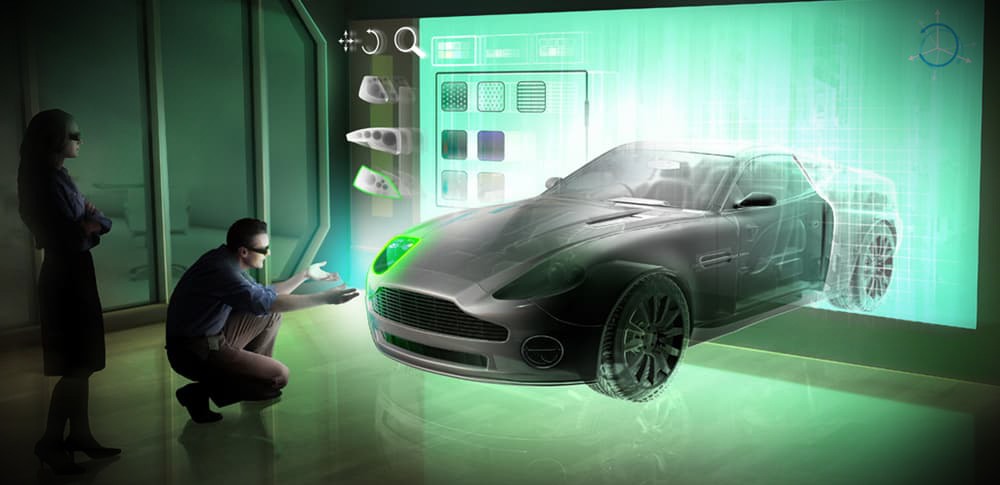
\includegraphics[width=1.0\textwidth]{figures/nvidia-3d-vision-pro}
		\caption[Promotional image for the NVIDIA 3D Vision Pro technology]{Promotional image for the \textit{NVIDIA 3D Vision Pro} technology (\textit{source:} \cite{Gizmag.2010}).}
		\label{fig:3dVisionary}
\end{figure}

Since the early years of science fiction story telling in books and movies, the concept of enriching our environment with digital information and other virtual content fascinates humanity. Movie franchises like \textit{Star Trek} and \textit{Star Wars} introduced unbelievable technology to a broad audience. First and foremost stories of space travel via huge ships with the help of fantastic inventions are meant to be entertaining. Having said that, the writers try to put the sci-fi technology into the context of a possible future science to make the shows more believable and exciting. The \textit{Holodeck}\index{Holodeck} in Star Trek is a good example of such an attempt. The Holodeck is an  environment simulator, which creates virtual worlds with the help of holographic projections in special rooms. It is used by the crew of the Enterprise for entertainment but also for training purposes. Although we can not yet imagine how to create a holographic image with which we can interact in such a way, the idea of fully accessable virtual worlds, the \textit{virtual reality} (see \autoref{sec:VAR})\footnote{The Holodeck may fall into the category of either a VR or an AR environment. The projection creates virtual content and the users can fully interact with it. The Holodeck itself is just a blank room, which makes the people interacting with it the only \enquote{real components}. Therefore there is no virtual overlayed \enquote{real} environment but only the virtual world the users have access to. According to the definitions used in this thesis (\autoref{sec:VAR}), the Holodeck is more of a VR application.}, has been a heavily researched field since the mid 19th century (compare with \cite{Nasa.2009}, \cite[p.3]{Toennis.2010}, \cite[p.19 et seq.]{Doerner.2013} and \cite[p.4 et seq.]{Burdea.2003}).

However, in many ways the actual development of the required hardware and software is still in its early stages (see \autoref{sec:history} for a historical overview of this topic), and although the concept was promising, we spent too many years \enquote{trapped} in the second dimension, leading to disappointments and the loss of people's confidence in the technology.

But with the improvement of sensors, graphics computation and displays the development of AR and VR applications can finally make significant progress. While the entertainment industry seems to be the most anticipated and closely followed development by the general public, the research on \textit{computer vision}\footnote{An explanation on this topic can be found at \autoref{ssec:cv}.} is still mostly driven by the military, NASA, the medical field and other technical industries. The tracking, recognition, analyzation, and finally digitization of real world objects and persons are important research fields for 3-D computer vision. In the future, surgeries will be fully supported with an AR overlay which displays the insides of the patient in real-time\footnote{The technology, with which the surgeons can see in real-time stereo vision with the help of tracking markers and stereoscopic glasses, is already far advanced (see \cite{Lowe.2016} for more examples).} and military drones could be able to distinguish between civilian and military buildings. Autonomous cars will reduce the risks on the streets and customers could design their individualized products interactively (see \autoref{fig:3dVisionary} for the vision NVIDIA presented in their promotional image for their new 3-D technology).

Despite all the recent successes, researchers are still struggling to reconstruct 3-D shapes and analyze/ interpret images in their entirety. But why is it so difficult? Why are people still disappointed? This misperception can be dated back to the early stages of robotics and artificial intelligence, in which it was initially believed that computer vision would be the easiest step to achieve (\cite[p.5]{Szeliski.2011}). 

Richard Szeliski, author of \textit{Computer Vision - Algorithms and Applications}, calls it an \enquote{inverse problem}: we try to find a solution on a basis of insufficient information provided by our imperfect technologies. We must turn to a physics- and mathematics-based approach to fill in these missing gaps and to create better \textit{models} of our real world. These include, for example, the modeling of shading and light reflection or the computation of the natural movement of colliding objects (compare with \cite[p.3 et seqq.]{Szeliski.2011}).  

In conclusion, the problems with computer vision can be broken down to mathematical algorithms, which are still merely models and subject to a multitude of errors. Some of these algorithms shall be the topics of this thesis.  
 
\begin{itemize}
\item computer vision 

\item optronis, highspeed cams --> why?
\end{itemize}
 
\section{About this thesis}
The present thesis is submitted in fulfillment of the requirements for the degree of Master of Science in \textit{Computer Science in Media} of the faculty of \textit{Digital Media}. The high-speed cameras and their software components as well as technical support were provided by the company \textit{Optronis}.

--> fragestellung, aufgabenstellung, zu erreichender grad, wieso highspeed (lack of data --> come back to inverse problm), optronis --> on consumer level \\
--> the goal for consumer market is to make all easy and cheap 
--> the goal for industry is to connect virtual and real world content seamlessly  

- could use ideal images - already a lot of studies --> not real

\textit{Optronis}\index{Optronis} is a German company which is specialized in the field of ultra-fast optical measuring systems since 1986\footnote{Check Optronis' webpage for more detailed information about the company and its products: \url{http://www.optronis.com}}. Their products are used for research and science in several fields. Both their high-speed cameras for precision measurements and their streak camera technology, which makes photons visible, help monitoring and analyzing processes that are otherwise invisible for the human eye (\cite{Optronis.2016}).

This thesis is loosely linked to my bachelor's thesis, in which the \textit{Oculus Rift}, a head-mounted display\footnote{More information about head-mounted displays can be found in \autoref{sec:VAR}. The  bachelor's thesis is digitally attached (in German).}, was transformed into an AR device with the help of two webcams. The software was developed in \CS and the shading language \textit{Cg} in the \textit{Unity Engine} (\cite{Haefele.2014}).     

\todo{--> zeitplan, --> vorgehensweise}
\todo{	- Leitfaden, worauf auch thesis aufgebaut ist:
		3 Levels of visual processing system (see Algorithms and Applications)}

\begin{itemize}
\item Methodik der thesis
\item Kapitelaufbau: hangelt sich an Pipeline lang - v.a. grundlagen und Implementierung
\item Background: basic definitions/ wording and historical background
\item related works: paper, matlab examples, theses
\item Math. principles: algos and calculations
\item Implementation: 
	\begin{itemize}
	\item first final pipeline, also includes some more math. principles that are more specific
	\item sessions and their results
	\item summarize problems / results
	\end{itemize}
\item closure: ...
\item glossar, why?
\item appendix:  calibration pattern included, from calibr. toolbox, experimental sessions documentations
\item the sequences not completely included since they are too big
\end{itemize}


\begin{figure}[htbp]
		\centering
		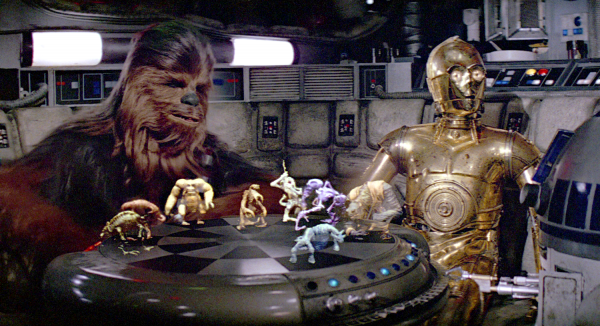
\includegraphics[width=0.8\textwidth]{figures/starWars}
		\caption[Bla]{Bla (\textit{source: 20th Century Fox ?} bla).}
		\label{fig:starWars}
\end{figure}
%\todo{another example for AR: star wars chess --> make two graphics with holodeck and star wars chess http://cdn.slashgear.com/wp-content/uploads/2014/06/falco-600x326.png }

		% Preface & about this thesis

\chapter{Background}\label{c:Background}
\label{c:Background}
\section{Definitions}
This section covers and differentiates between the basic non-mathematical definitions and terms used in this thesis.

\subsection{Virtual and Augmented Reality}\label{sec:VAR}
The words virtual reality (VR) and augmented reality (AR) can be constantly read in the recent news all over the internet and other media. However, they are used in various contexts and are often defined differently. The definition used in this thesis is therefore only one small aspect of the whole field and should help to differentiate between the two concepts. 
\subsubsection{Virtual reality}
Virtual reality\index{Virtual reality} can be defined as \enquote{an electronic simulation in which images are generated in real time (...) from a stored database and displayed in such a way as to facilitate real-time interaction with the database (...).} \cite[p.148]{Latham.1995}

A virtual reality application uses a combination of software and hardware to let the user experience immersion, interaction and imagination (the three I's of virtual reality) in a virtual world. Whereas the first two I's should be clear and understandable, the last one is often underrated or even left out. Since virtual reality only counts on virtual content and given the fact that computer graphics are still not a perfect representation of our \enquote{reality}, the user's imagination is a very important aspect of an application (\cite[p.3 et seq.]{Burdea.2003}).

Typically, a common computer game can not be classified as a virtual reality application unless it includes the collection and usage of other data than only the keyboard and mouse inputs. For this purpose, a VR application often comes with other interfaces such as a head-mounted display (HMD)\index{Head-mounted display} \footnote{The idea of a HMD started with Morton Heilig's  \index{Morton L. Heilig} U.S. patent in 1960 (see \cite{Heilig.1957}). Recent popular models include the \textit{Oculus Rift} (see \cite{Oculus.2016})\index{Head-mounted display!Oculus Rift} and \textit{Google Cardboard} (see \cite{GoogleDev.2016})\index{Head-mounted display!Google Cardboard}. The HMD tracks, amongst other things, the head position and its movement and displays the stereo image.}. An imaginary example for a perfect virtual reality environment is Star Trek's Holodeck, as mentioned before (\autoref{sec:preface}).

\subsubsection{Augmented reality}
\begin{figure}[htbp]
		\centering
		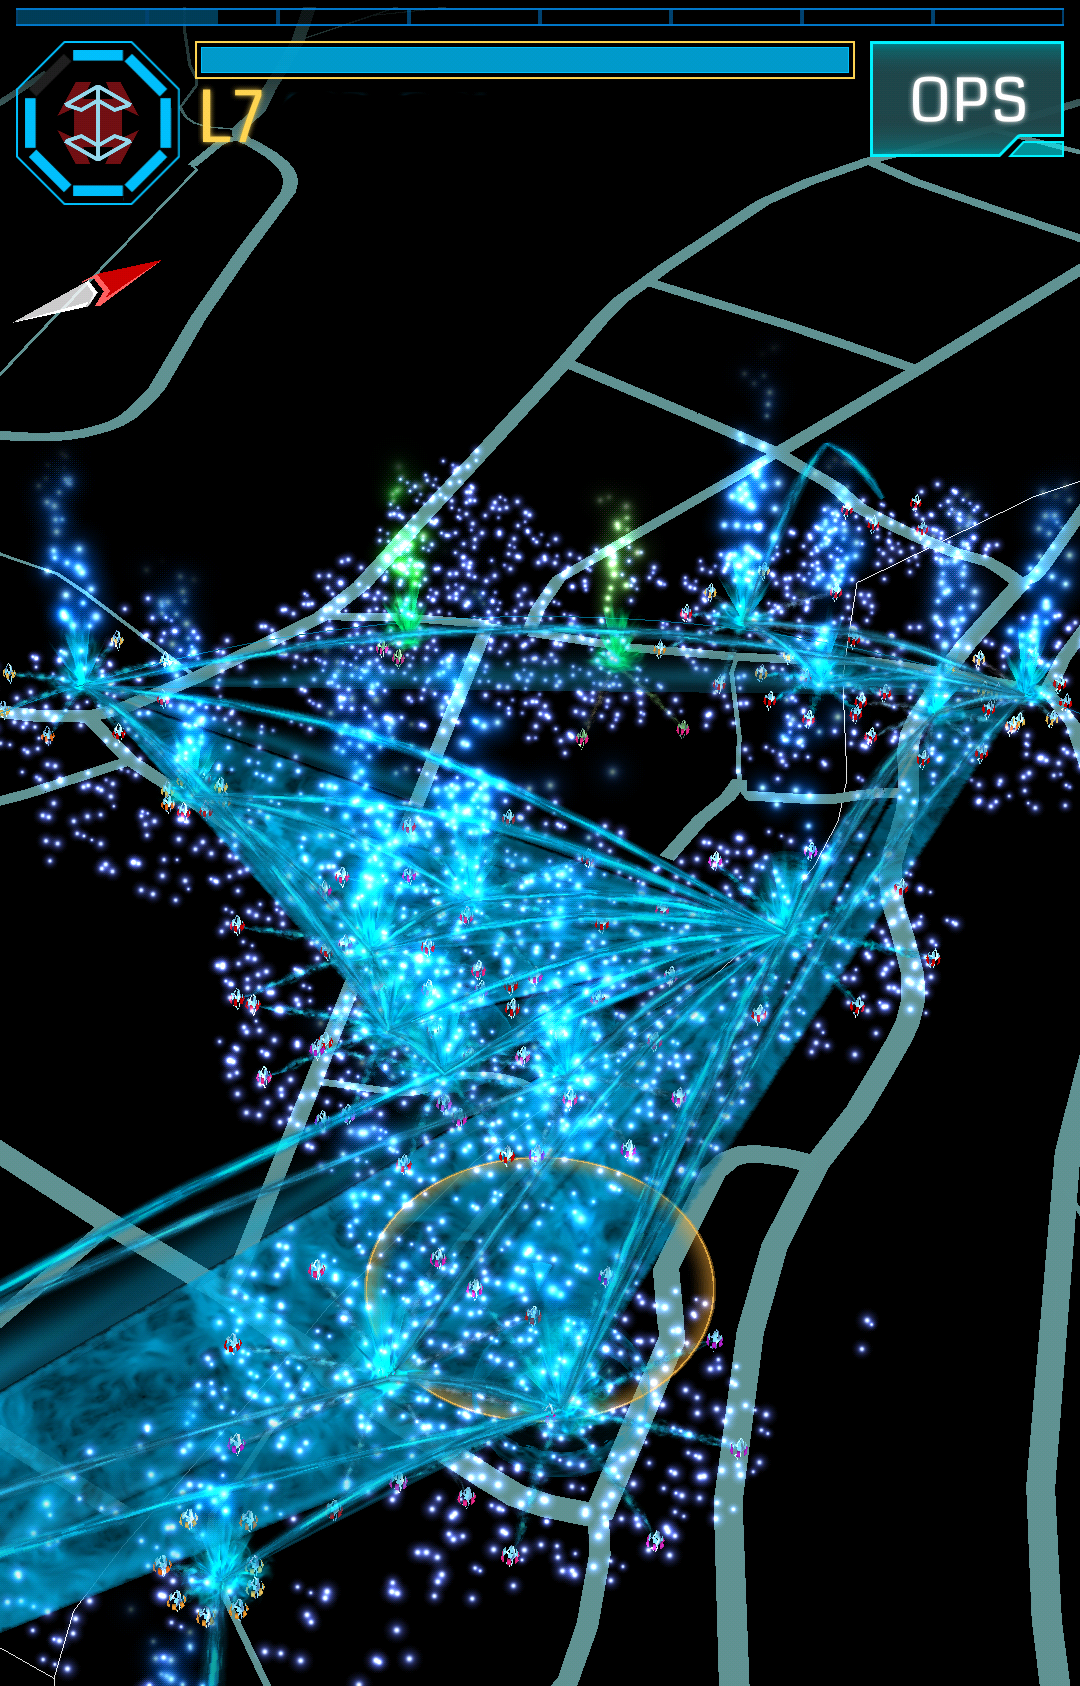
\includegraphics[width=0.4\textwidth]{figures/Ingress}
		\caption[Screenshot of the mobile AR game Ingress]{Screenshot of the mobile AR game Ingress showing the portals around the Hochschule Furtwangen University (\textit{source:} \cite{Haefele.2014}).}
		\label{fig:Ingress}
\end{figure}
In comparison to virtual reality, augmented reality \index{Augmented reality} extends our \enquote{real world} with virtual (digital) content, which must be embedded seamlessly to provide a fully immersive experience. The users can interact with virtual objects and can be provided with relevant additional information about their environment. The virtual data is computed in real-time and is displayed as an overlay on top of the \enquote{real world} in front of the user's eyes. AR highly relies on its technologies. Relevant topics, amongst others, are object recognition, location tracking, interfaces\footnote{A common interface for AR was and still is the head-up display (HUD)\index{Head-up display}, often used for military application (see \cite[p.6]{Burdea.2003}). But also immaterial displays, such as fog screens, are researched (see \cite[p.25 et seq.]{Toennis.2010}).} and real-time computation (compare with \cite[p.1 et seqq.]{Toennis.2010}). 

The game \textit{Ingress}\index{Ingress} by \textit{Niantic, Inc.} (see \autoref{fig:Ingress} for a screenshot), in which two factions fight over virtual portals, is an example for a location-based mobile AR game. The portals, which are linked to real places all over the world, and other game functions are displayed on the user's mobile device in real-time. The users travel to these real places to conquer or defend the portals in the name of their faction (\cite{Niantic.2016}). 

\subsection{Computer vision}\label{ssec:cv}
Computer vision\index{Computer vision} (also referred to as \enquote{machine vision}) is the \enquote{automated extraction of information from images} (\cite{Lowe.2016}). It also refers to a whole field of science, which combines several disciplines\footnote{Among which are mathematics, computer science, as well as phsyics, the psychology of perception and the neuro sciences (\cite[p.xi]{Hartley.2011}).} to research how to make a computer see. Computer vision is differentiated from the wide field of image processing, in which images are processed in different ways to produce new images (compare with \cite{Lowe.2016}).
 
As already stated in the preface, the visual modeling of perception was, for many years, underestimated by scientists studying Artificial Intelligence. Although it is still unclear whether computer vision should be modeled on the basis of biological systems, understanding how biological vision in general, and human depth perception in particular function, seems to be a necessity\footnote{Attempts to find new approaches have not yet been successful.} (compare with \textit{Oliver Faugeras'} foreword in \cite[p.xi]{Hartley.2011}). For this a short overview shall be given in \autoref{ssec:hv}.  

One of the research fields in Computer Vision is the 3-D reconstruction from image data (other fields are listed in \autoref{ssec:Today}). Two important procedures to reconstruct scenes are \textit{structure from motion}\index{Structure from motion} and \textit{stereo correspondence} algorithms. The former uses multiple views of one or more cameras to reconstruct scenes and the latter is described in more detail in the following chapters, since it was used in this thesis.

\subsection{Human Depth Perception}\label{ssec:hv}
Our three-dimensional perception is actually based on a two-dimensional image which is projected onto our retina, but from these 2-D images we are still able to get information about how far away an object is. This information is called \textit{depth cues}\index{Depth cues}, whose connection to the actual depth of field we learn from experience. Depth cues need to be applied to stereoscopic videos to create more accurate depth results (\cite[p.226]{Goldstein.2015} and \cite[p.28]{Hottong.2009}). 

These depth cues can be classified into three different groups (freely adapted from \cite[p.226 et seqq.]{Goldstein.2015} and \cite[p.28 et seqq.]{Hottong.2009}):
\begin{description}
\item [i Oculomotor depth cues\index{Depth cues!Oculomotor depth cues}]\hfill \\ These cues provide depth information for objects which are in closer range (one meter or below). Our brain receives and analyzes feedback from the eye muscles which are contracted differently depending on the distance of the object which gets focused on. We can subconsciously \textit{feel} the muscles' contraction and draw conclusions from it. The oculomotor cues are based on two factors: \textit{accommodation}\index{Depth cues!Accommodation} and \textit{convergence}\index{Depth cues!Convergence}\footnote{The former is based on the contraction of the ciliary muscles, which allow the lens of the eye to take on different shapes in order to change their focal length. The latter uses the information of the eyes' movement as they converge on a moving object to estimate distances.}.
\item [ii Monocular depth cues\index{Depth cues!Monocular depth cues}]\hfill \\ As the name suggests these depth cues can be perceived even with only a single eye (which is one of the reasons that people with only one eye can still perceive depth). They use the previously mentioned accommodation in combination with \textit{pictorial} as well as \textit{movement-produced depth cues} to estimate depth.
	\begin{description}
	\item [Pictorial depth cues]\index{Depth cues!Pictorial depth cues}\hfill \\ Information about depth which can be displayed in a two-dimensional picture. Among them are (\cite[p.227 et seqq.]{Goldstein.2015}):
		\begin{itemize}
		\item \textit{Occlusion}\index{Depth cues!Occlusion}: An overlapped object seems to be further away than the object in front of it. We can not determine the absolute distance of these objects, since these are only relative cues.
		\item \textit{Elevation}: Relative to the horizon we perceive objects which are closer to it as further away than the ones below or higher than it. 		
		\item \textit{Relative and familiar size}: Two objects with the same size change their perceived size according to their position relative to the observer. Objects which are closer appear larger and vice versa. We use our experience to estimate sizes of objects and their distances to us (\autoref{fig:Perugino} shows the difference in sizes of the people which illustrates relative sizes).
		\item \textit{Perspective}\index{Depth cues!Perspective}: Parallel lines converge in the distance and meet in infinity. This concept was often used by artists of the Renaissance to create the optical illusion of depth in their paintings (see \autoref{fig:Perugino} in which the lines converge towards one vanishing point).
		\item \textit{Aerial perspective}: Objects in the far distance appear to be hazy\footnote{In computer games this phenomenon is often called \textit{distance fog}.} and often times have a blue tone with lower contrasts (note that the painter in \autoref{fig:Perugino} used cool colors for distant objects and warmer colors for the foreground).
		\item \textit{Texture gradient}: Textures appear less detailed the further they are from the observer. At the same time elements appear more dense relative to the distant of the viewer.  
		\item \textit{Shading}: Shadows help us to determine positions and they amplify the three-dimensional appearance of objects. 
		\end{itemize}
	\item [Movement-produced depth cues]\index{Depth cues!Movement-produced depth cues}\hfill \\ With the movement of our head or our whole body we receive more cues to determine depth. One of the most important cues is the \textit{motion parallax}\index{Depth cues!Motion parallax}. This depth cue occurs when we see closer objects pass us in a faster speed and more distant objects in a slower pace. It is also often used in 2-D side-scrolling video games (also called \textit{side-scrollers}\index{Side-scroller}) to illustrate depth of field.
Another movement-produced depth cue is the occlusion of objects due to movement (\cite[p.231 et seq.]{Goldstein.2015}).
\end{description}

\begin{figure}[htbp]
		\centering
		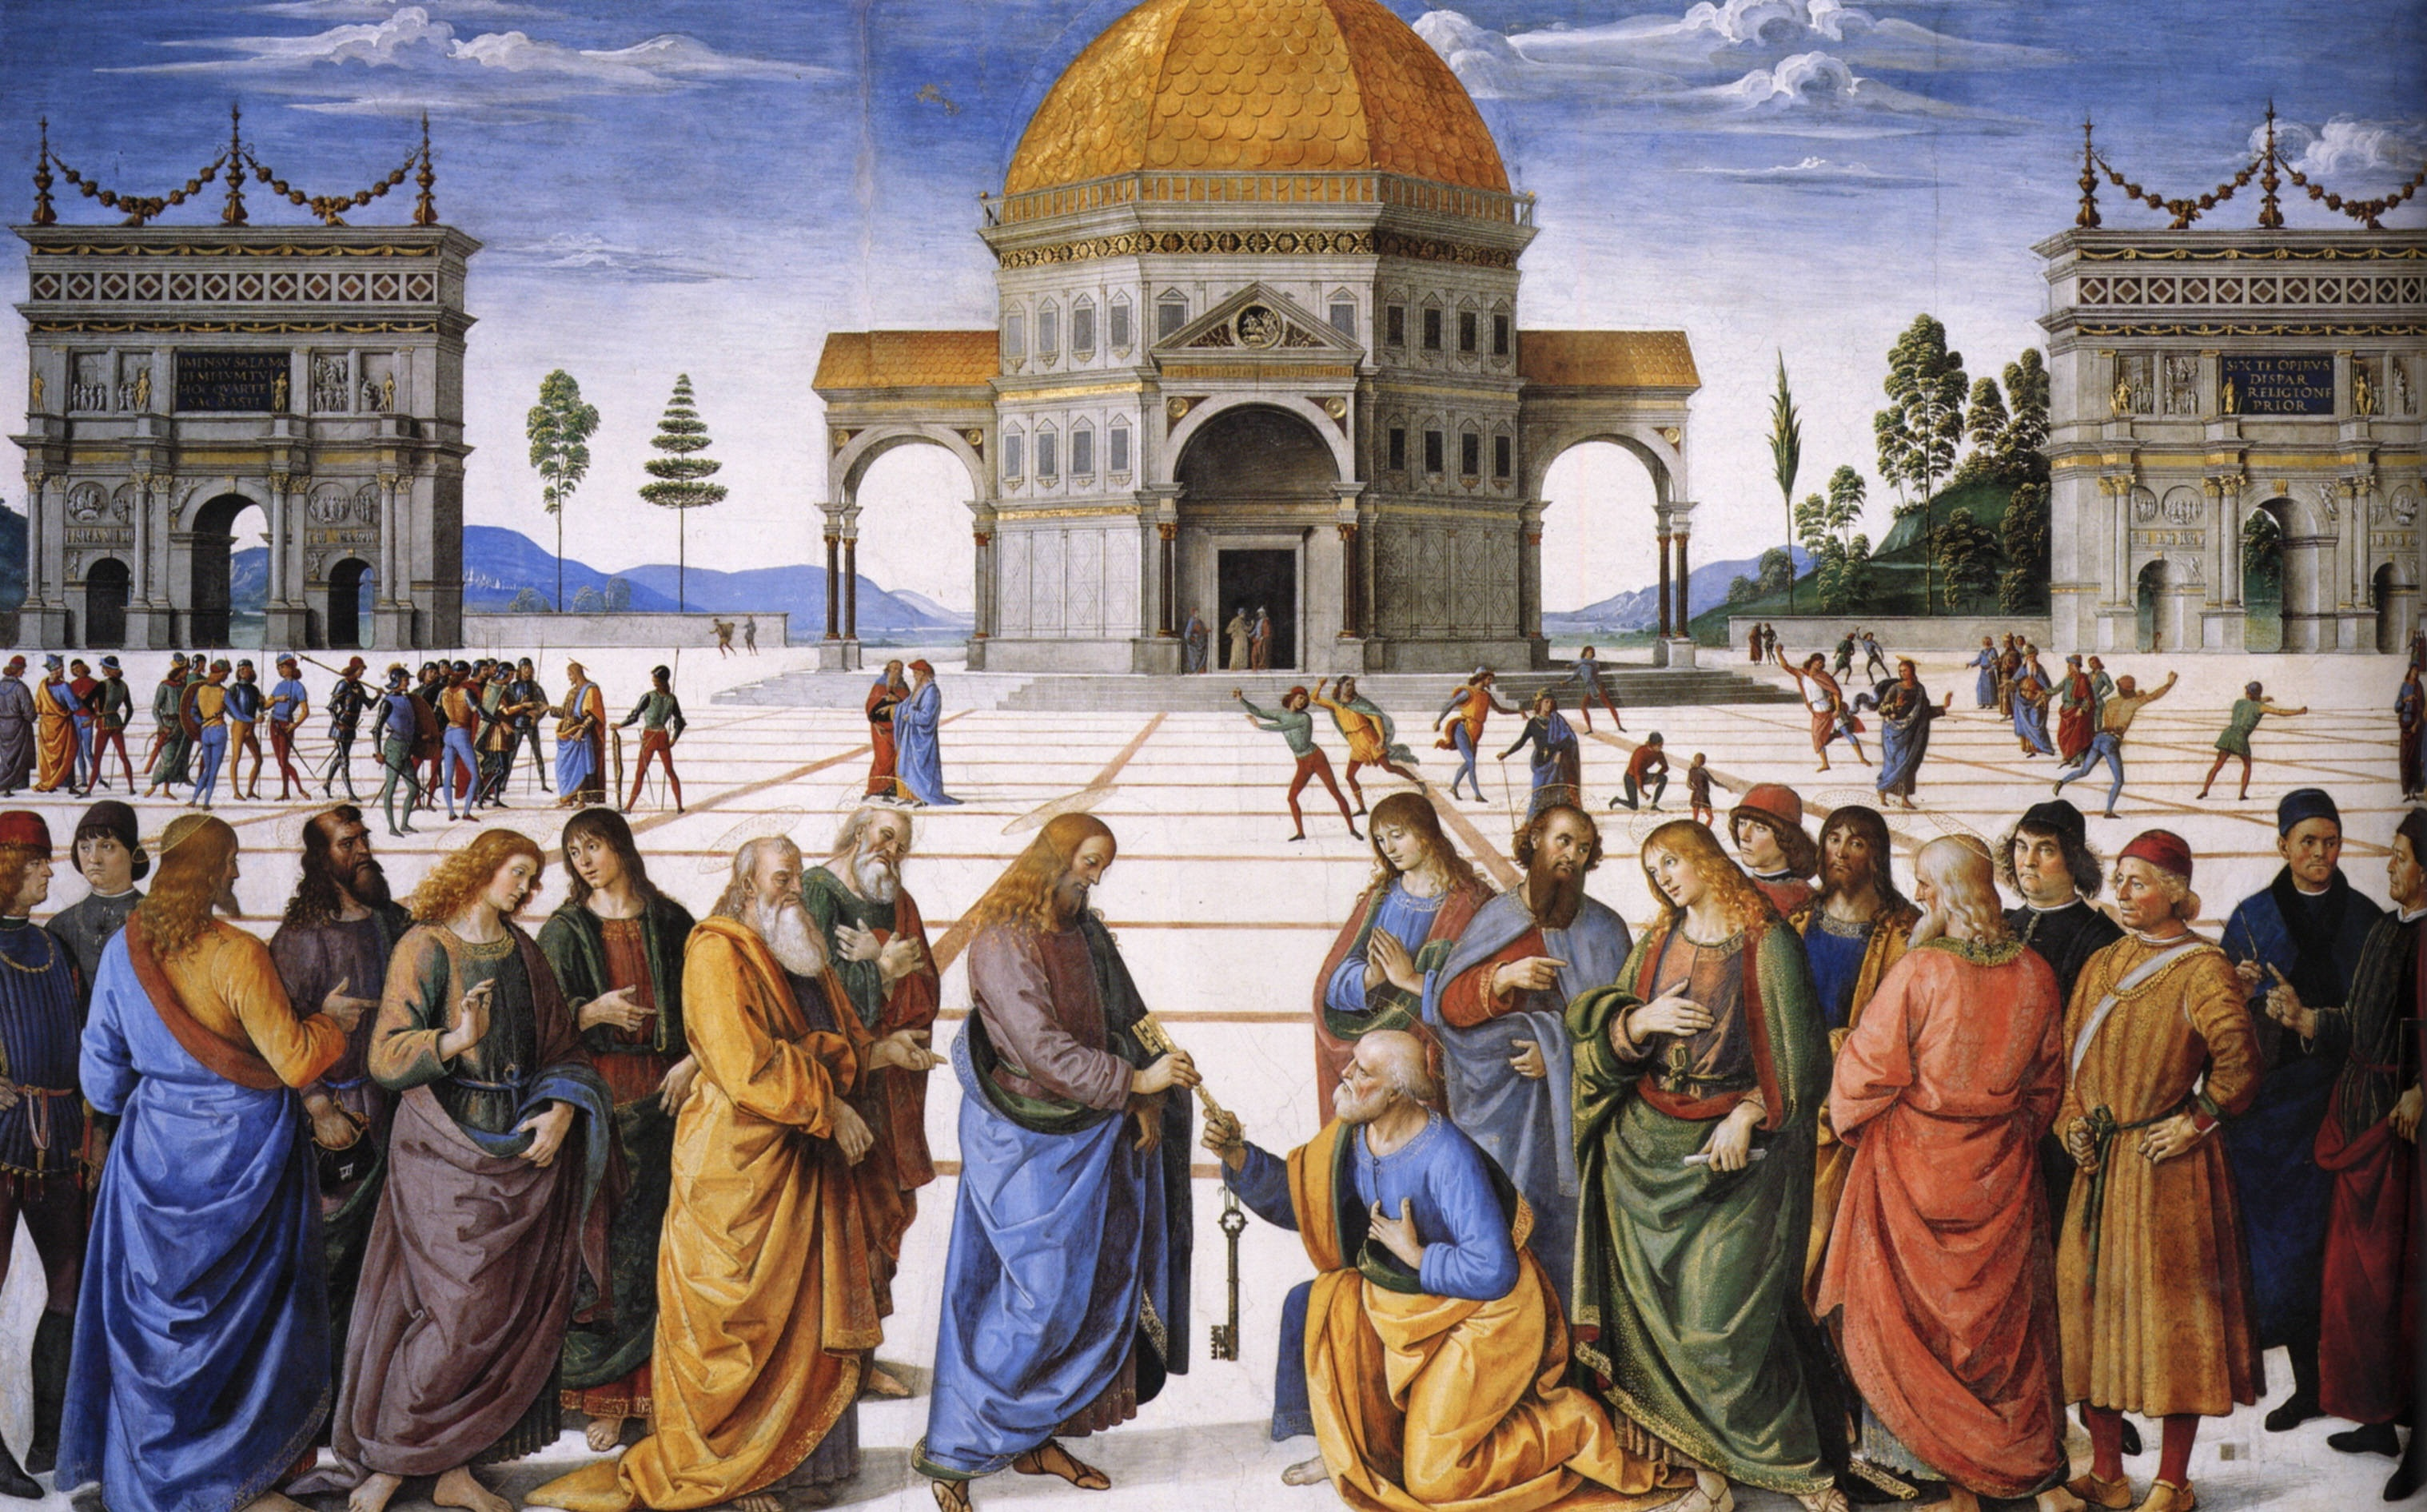
\includegraphics[width=0.8\textwidth]{figures/Perugino-San_Pedro}
		\caption[Pictorial depth cues in Pietro Perugino's fresco \textit{Entrega de las llaves a San Pedro}]{Pictorial depth cues in Pietro Perugino's fresco \textit{Entrega de las llaves a San Pedro} in the Sistine Chapel, Vatican City, 1481-1482}
		\label{fig:Perugino}
\end{figure}

\item [iii Binocular or stereoscopic depth cues\index{Depth cues!Binocular depth cues}]\hfill \\ Stereoscopic depth cues are stimuli for which we need both eyes to experience depth of field. They mainly take the differences between the right and the left image seen by our eyes into account, which makes the interpupillary distance the bases of the stereoscopic vision\footnote{Computer vision algorithms use these principles as a model for creating or analyzing depth with the help of two or more cameras (see \autoref{c:Math} for more details).}.
\end{description}
 		% Overall definitions & History
\section{History}\label{sec:history}
\subsection{First developments}
In the late 50s of the 19th century \textit{Morton Leonard Heilig}\index{Morton L. Heilig} dreamed about the revolution of cinematic story telling and designed with his \enquote{stereoscopic-television apparatus for individual use}\index{Head-mounted display!Stereoscopic-television apparatus for individual use} the first head-mounted display (see \autoref{fig:Heilig}). The helmet was planned to display stereoscopic images, play surround sound and even add smell to the sensory experience, but was never actual built. His ideas were ahead of their time and could not yet be realized with the technology of the time (compare with \cite[p.3]{Toennis.2010} and \cite[p.4 et seq.]{Burdea.2003}). 

In the decades to follow, several attempts to bring input and display devices for virtual reality onto the consumer market failed due to their high costs and their lack of software. In 1992, \textit{Jaron Lanier}\index{Jaron Lanier} and his company \textit{VPL Research} released the \textit{DataGlove}\footnote{The \textit{datagloves}\index{Dataglove} (also called \textit{wire-} or \textit{cybergloves}) are another step into more immersive input devices, since hand gestures can be directly used to interact with the virtual world.}\index{Dataglove!DataGlove} at the unaffordable prize point of \$9000 USD. The low number of games for \textit{Nintendo's} cheaper \textit{PowerGlove}\index{Dataglove!PowerGlove} led to its discontinuation in 1993 soon after its introduction (\cite[p.8 et seq.]{Burdea.2003} and \cite[p.19 et seq.]{Doerner.2013}).

\begin{figure}[htbp]
		\centering
		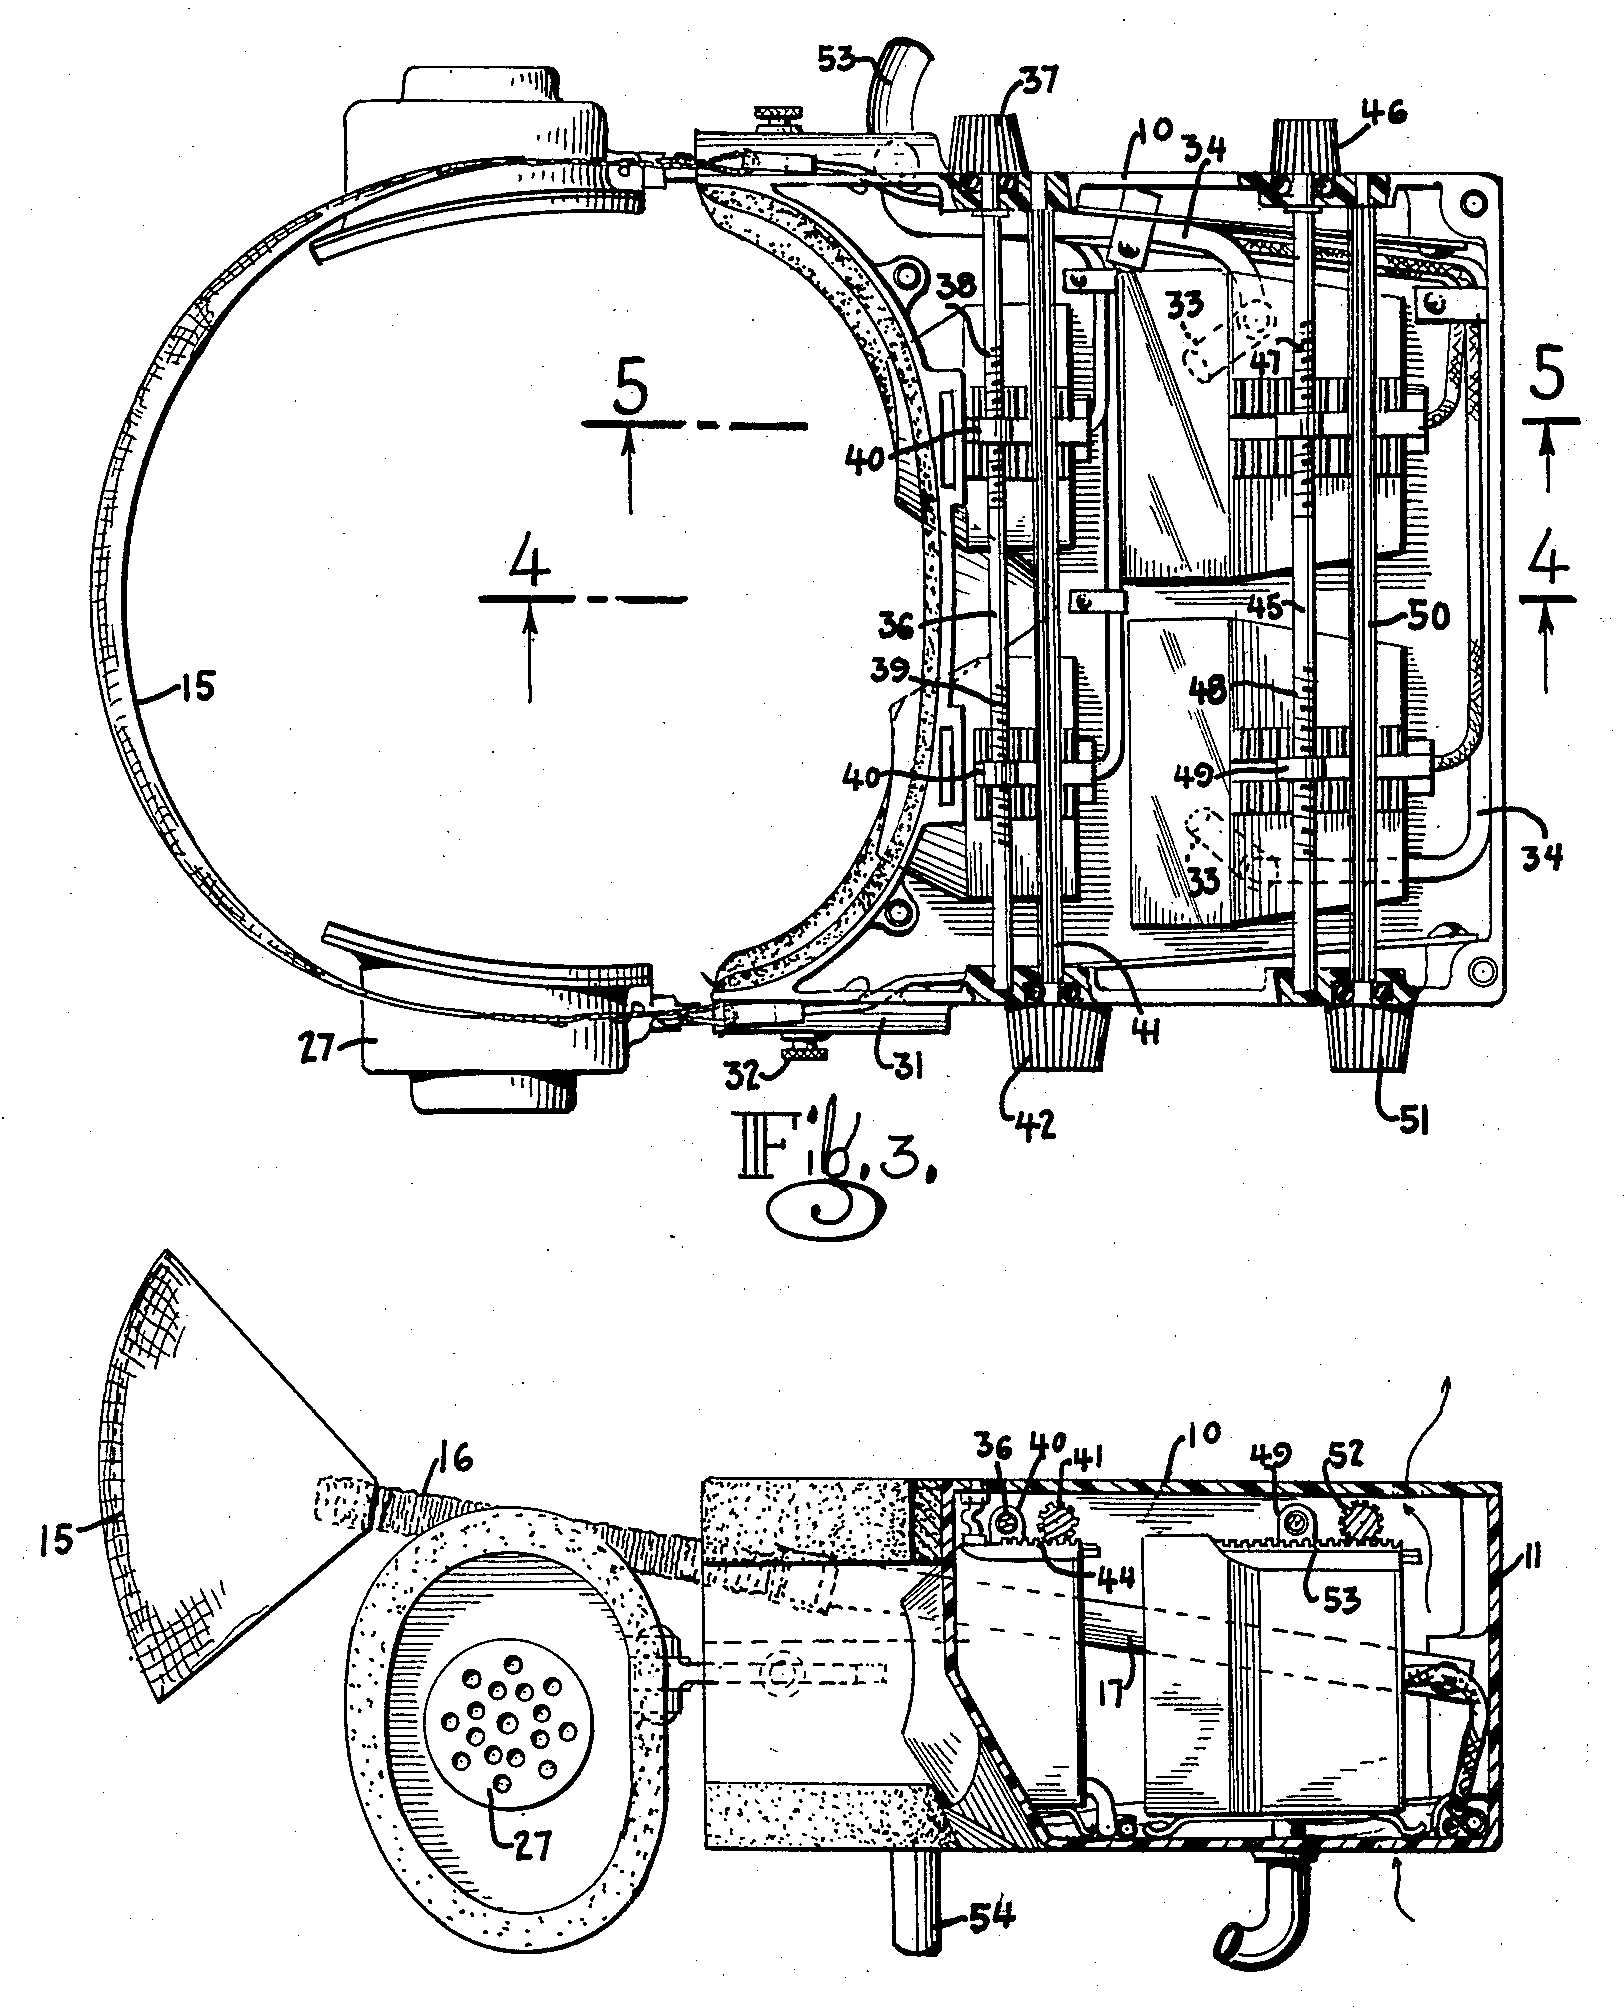
\includegraphics[width=0.4\textwidth]{figures/Heilig_HMD}
		\caption[Stereoscopic-television apparatus for individual use]{Morton Heilig's stereoscopic-television apparatus for individual use (\textit{source: \cite{Heilig.1957}}).}
		\label{fig:Heilig}
\end{figure}

\subsection{Disappointments}
The 80s and 90s were characterized by heavily marketed products, that ultimately disappointed the users and failed to live up to the \enquote{mediahype}. The expectations for virtual reality applications were too high and the technological development was not fast enough. The hardware was too costly\footnote{The fastest graphics system, the \textit{Reality Engine} by \textit{Silicon Graphics}, cost \$100,000 USD at its release in the 1990s(\cite[p.10]{Burdea.2003}).}, the market for VR was too small and there were no investment funds available for companies. These deficits led to the bankruptcy of many companies and caused a serious crisis for the VR industry (\cite[p.10]{Burdea.2003}). 

\todo{spell-check from here}
Meanwhile the development of virtual reality \todo{... the role of military and NASA, sensor improvement, ...} \\

With the improvement of computer hardware in the late 90s, the graphics computation began to meet the requirements for VR and the hardware was finally affordable for consumers (\cite[p.10 et seq.]{Burdea.2003}, \cite{Doerner.2013} and \cite[p.3]{Toennis.2010}).

\subsection{Today's usage of computer vision}\label{ssec:Today}
Fortunately, recent successes in the industry were made and the computer vision plays an increasing role in many fields. \textit{David Lowe}, Senior Research Scientist at Google Seattle, has enlisted the following categories of today's important industrial applications of computer vision\footnote{Although he states that his list is not complete and not up-to-date, it can be used as an overview. Go to his homepage to read more about specific applications: \cite{Lowe.2016}} (freely adapted from \cite{Lowe.2016}): 

\begin{description}
\item [Automotive driver assistance and traffic management,]\hfill \\ such as warning vision systems and real-time traffic management.
\item [Eye and head tracking,]\hfill \\ which is also included in head-mounted displays.
\item [Film and video,]\hfill \\ e.g. tracking of the ball in sports for sport-analyzing or motion tracking systems for animated movies.
\item [Gesture recognition,]\hfill \\ such as full-body motion sensing with the Mircosoft Kinect and gesture recognition as computer inputs for gaming or other computer-related activities.
\item [Industrial automation and inspection,]\hfill \\ like systems for inspection and process control in the electronic or food and agriculture industry. 
\item [Medical and biomedical,]\hfill \\ e.g. the detection and tracking of markers in real-time stereo vision for surgeons.
\item [Object recognition and AR for mobile devices,]\hfill \\ including real-time product recognition and image refinement applications, such as face-swapping apps.
\item [Photography,]\hfill \\ e.g. automated panorama stitching for multiple images.
\item [Safety monitoring,]\hfill \\ monitoring of areas to warn of accidents, e.g. in swimming pools.
\item [Security and biometrics,]\hfill \\ detection and counting of people for security purposes, fingerprint or license plate recognition.
\item [3-D modeling,]\hfill \\ 3-D scanners of objects or the 3-D reconstruction from a number of photographs. 
\item [Web and cloud applications,]\hfill \\ such as image retrieval based on content. 
\end{description}

Regarding all these examples, the entertainment industry seems to be the slowest candidate, which is partly owed to its users high expectations regarding the (graphics) quality. 
				% Historical Background
			

\chapter{Mathematical Principles}\label{c:Math}
(\cite{Hartley.2011})
\begin{itemize}
\item use Markus Mann - StereoCameraCalibration.pdf !!!!
\item and Camera Calibration for Stereo Vision.pdf
\item Disparity
\item Rectification
\item Triangulation?
\end{itemize}

\section{Coordinate systems}

\section{3-D reconstruction}

\subsection{Structure from motion}\label{ssec:SfM}
\subsection{Stereo matching}\label{ssec:stereoMatch}

\section{Disparity}

\begin{itemize}
\item Disparity Map
\end{itemize}

"Disparity refers to the distance between two corresponding points in the left and right image of a stereo pair. Obviously this process involves choosing a point in the left hand frame and then finding its match (often called the corresponding point) in the right hand image; often this is a particularly difficult task to do without making a lot of mistakes. A useful topic to read about when performing stereo matching is rectification. This will make the process of matching pixels in the left and right image considerably faster as the search will be horizontal."
(http://stackoverflow.com/questions/17607312/difference-between-disparity-map-and-disparity-image-in-stereo-matching)

\section{Rectification}
				% Math. Principles

\chapter{Related Works}\label{c:relatedWorks}
\chapter{Related Works}\label{c:relatedWorks}

\begin{itemize}
\item \url{http://www.hawkeyeinnovations.co.uk/} --> see description in \cite{Lowe.2016}
\item große family der computer vision applications: verweis auf background chapter --> todays usage (\autoref{ssec:Today})
\end{itemize}


		% State-of-the-Art
\chapter{Components} \label{c:Components}				% 	
\chapter{Components} \label{c:Components}
\section{Hardware} \label{sec:Hardware}
\todo{cams}

\section{Software} \label{sec:Software}
\todo{written in \LaTeX, other software follows:}

\subsection{Timebench} \label{ssec:Timebench}
timebench software (\url{http://www.optronis.com/en/about-us/innovation.html})

\subsection{MATLAB} \label{ssec:Matlab}
For the camera calibration as well as for the 3D reconstruction, the commercial platform \textit{MATLAB}\index{MATLAB} by \textit{MathWorks} was used. MATLAB is a software that is specialized in solving mathematical problems (especially matrix operations) and visualizing data. The MATLAB programming language is matrix-based and implements object-oriented concepts like classes and inheritance. The program comes with a large library of built-in toolboxes, which can be used to address many different engineering and scientific problems. Another of MATLAB's strengths lies with its active community, which provides costum scripts and discusses recent developments in the scientific field (\cite{MathWorks.2016}).

A large portion of the MATLAB community is involved in researching the algorithms that drive the field of multiple view geometry in computer vision (see \autoref{c:relatedWorks} for examples). MathWorks also implements new content on this topic regularly. 

The reasons stated above led to the usage of MATLAB as the development environment of choice in this thesis. Initially MATLAB R2015b was used, but due to newly added functions for data refinement (see \autoref{sec:refinement}) the software needed to be updated to MATLAB R2016a.
   
The 3D reconstruction was programmed and organized in one MATLAB script file. To get the needed stereo parameters an built-in toolbox was used, which will be discussed in the following sections. Documentation for all functions used and a step-by-step-guide can be found in \autoref{c:Implementation}.

One of the biggest problems with MATLAB is its documentation. Although it often provides good examples and a lot of details, it is not explicit enough in other important areas. Certain algorithms used in the built-in functions are often times not explained, making it difficult to find mistakes when the data output is unexpected\footnote{This \enquote{blackbox} problem with which you can not see how the output is created may be owed to the fact that MATLAB is (and is used as) a commercial software.}. The toolboxes often lack information as well, for example an explanation of how the pipelines work, which coordinate system is used, etc. These problems restrict the programmer quite a bit and force one to either find a work around or use third party programs. More details on the encountered problems can be found in the following chapters (especially \autoref{sec:Calibration} and \todo{add all chapters with big probs here}).

\subsubsection{Camera calibr. toolbox for matlab}
\subsubsection{Stereo calbr. toolbox for matlab}




\section{Experiment architecture} \label{sec:architecture}
versuchsaufbau --> visualize pipeline (?) + tatsächliche architecture 		% Architecture of Implementation, used software/hardware

\chapter{Experiments}\label{c:Experiments}	% Implemenation - code, results, ...
\label{c:Experiments}
The experiments chapter first describes the final experimental pipeline, which is divided into the Stereo Camera Calibration (\autoref{sec:Calibration}) and into the actual reconstruction (\autoref{sec:Reconstruction}) and secondly follows several experimental sessions to point out problems and results which occurred during the tests.

\section{Stereo Camera Calibration}\label{sec:Calibration}
The stereo camera calibration estimates the intrinsic and extrinsic parameters of a set-up of two uncalibrated cameras. The calibration is divided into first capturing image pairs of the checkerboard pattern (\autoref{ssec:PatternSequence}) and then estimating the parameters in the \textit{Stereo Camera Calibrator Toolboox}\index{Stereo Camera Calibrator Toolbox} in MATLAB (\autoref{ssec:estimateStereoParams}). The camera set-up used in the camera calibration must not be changed at all for the rest of the session: the sequence recorded for the actual 3-D reconstruction needs to have the same parameters.

\begin{figure}[htbp]
		\centering
		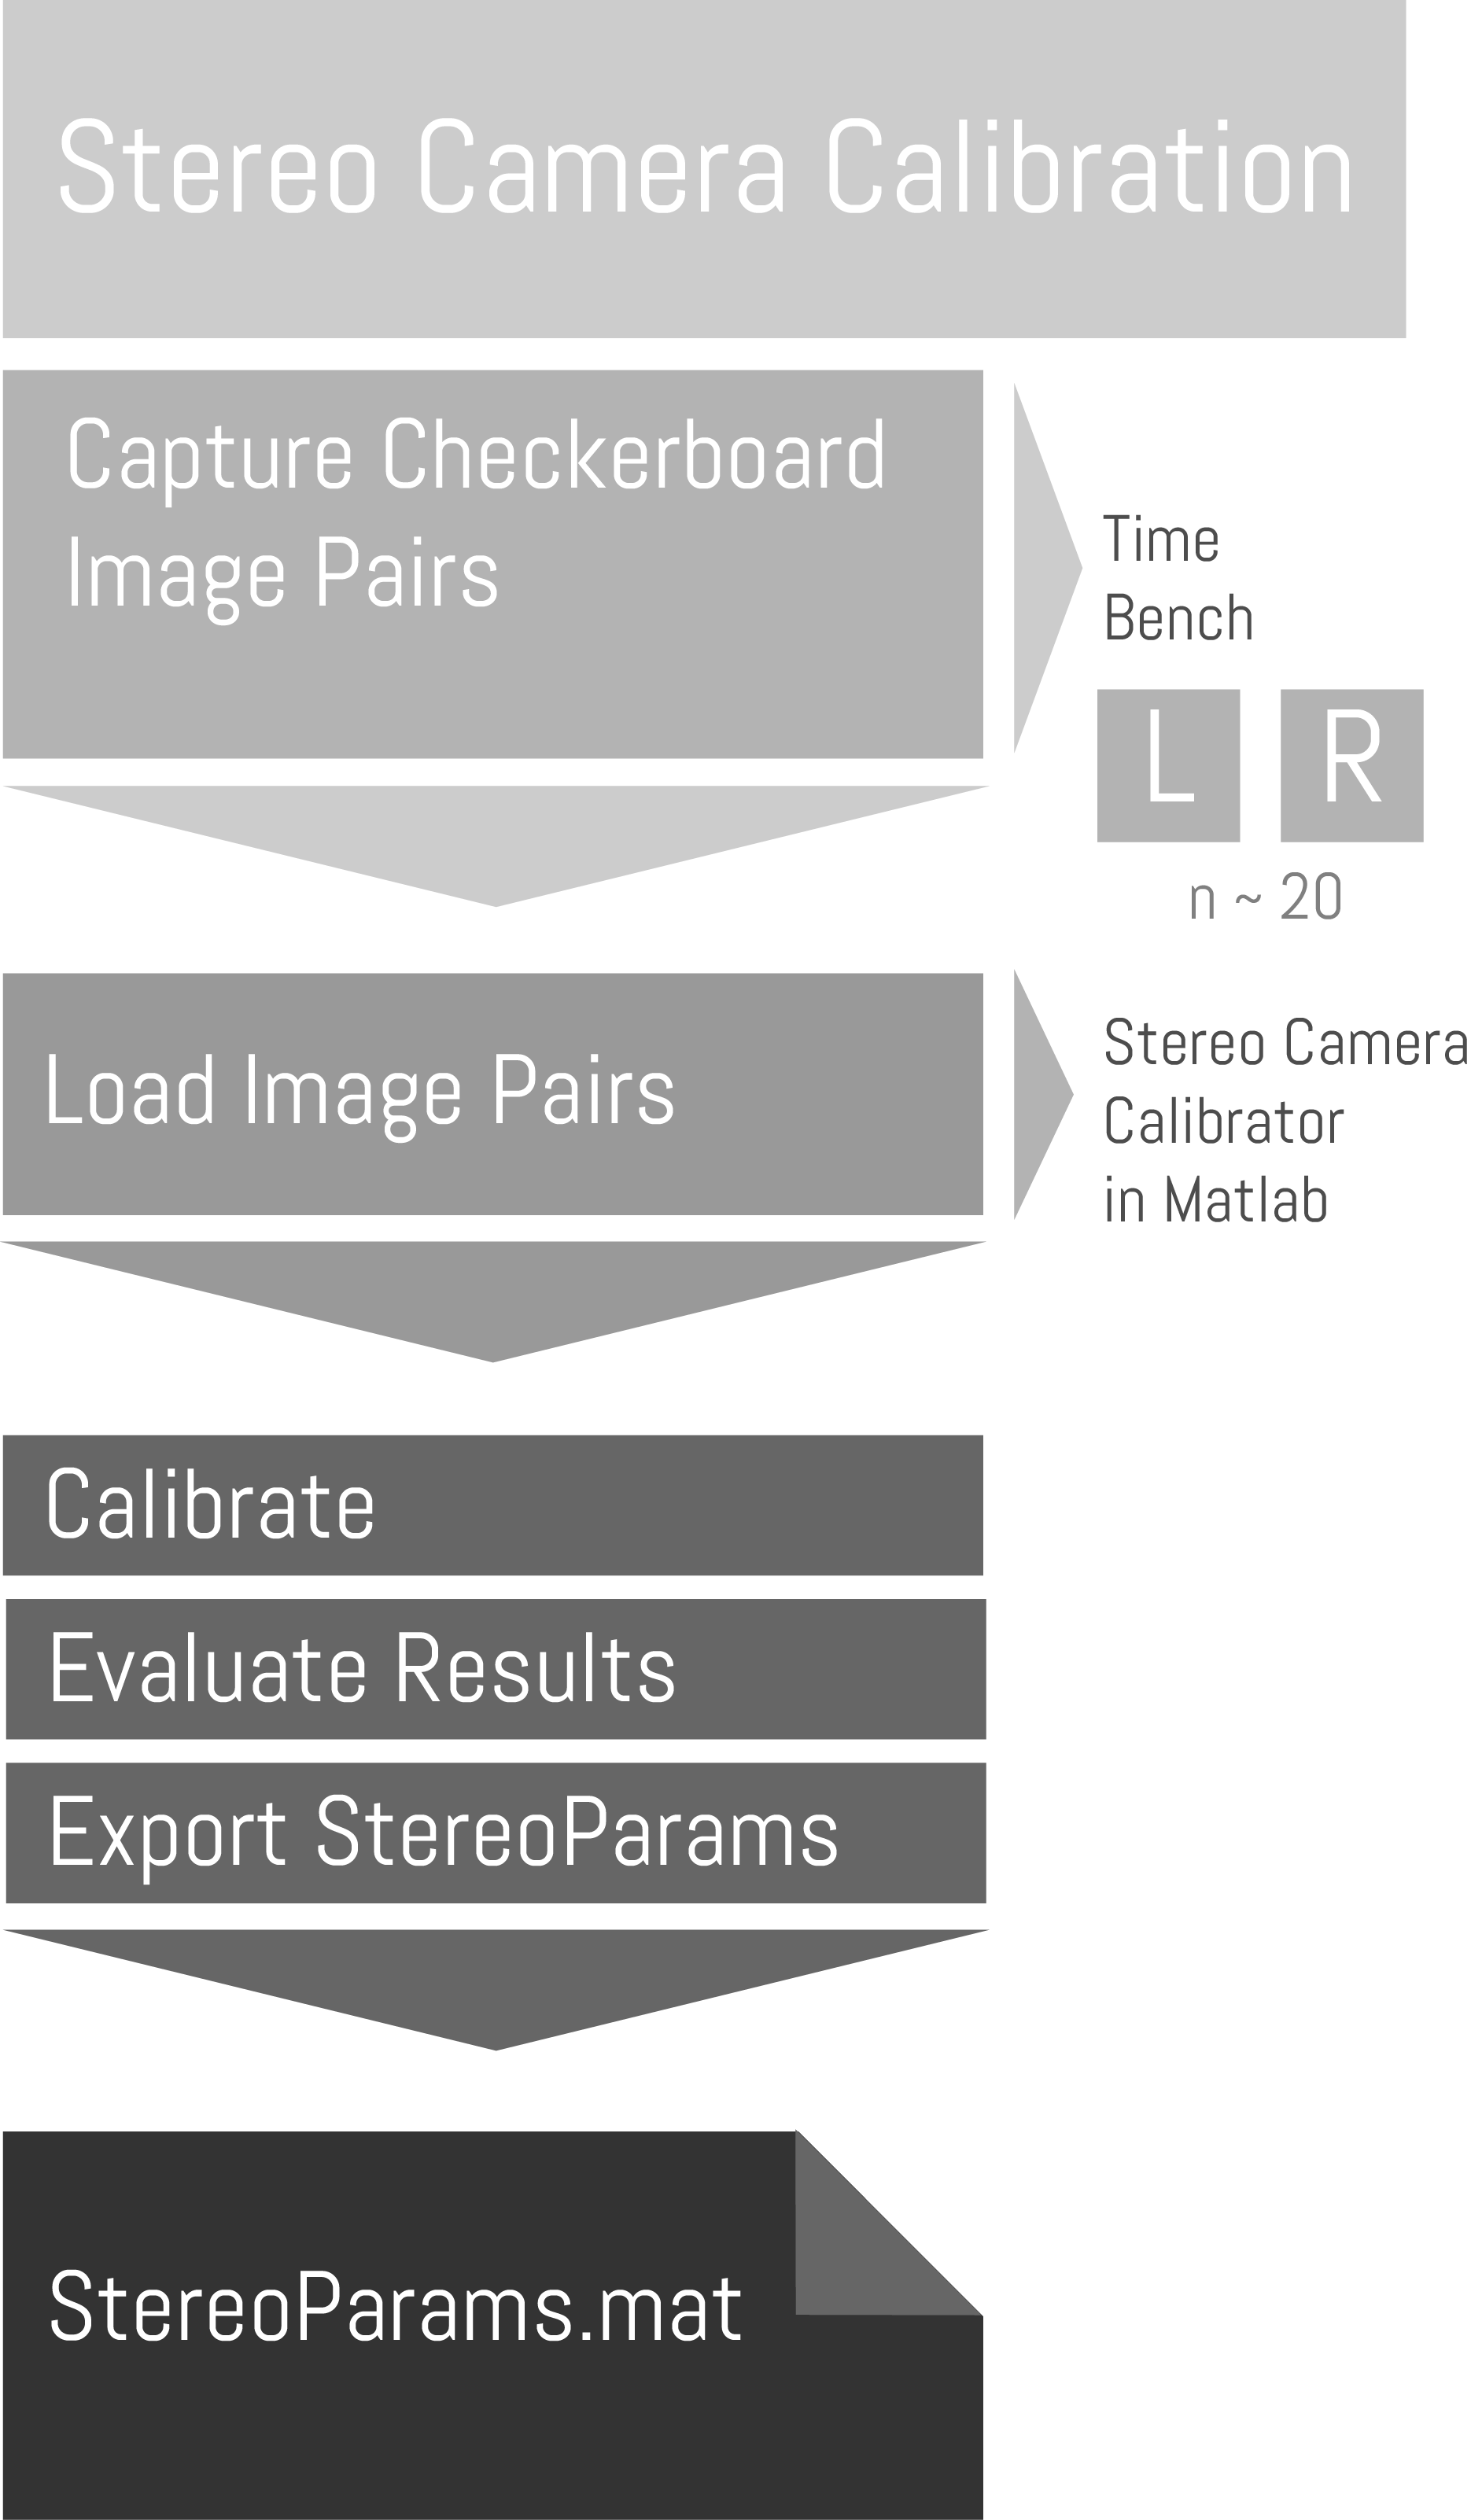
\includegraphics[width=0.7\textwidth]{figures/CameraCalibration}
		\caption[Steps of the stereo camera calibration]{Steps of the stereo camera calibration in TimeBench and in the Stereo Camera Calibrator for MATLAB, using $n$ image pairs.}
		\label{fig:stereoCamCalib}
\end{figure} 

\subsection{Capturing Sequence of Calibration Pattern in TimeBench}\label{ssec:PatternSequence}
The two cameras should be set-up next to each other with little to no rotation. For stereo display (anaglyphic display) the cameras need to be placed about 55 mm apart, which is about the distance between our eyes. Since this thesis does not create stereoscopic displays, the cameras' baseline is set to approximately 19 cm, which is the minimum distance the two cameras can be apart from each other due to the camera bodies.\footnote{Cameras which are placed farther apart from each other resolve in greater reconstruction accuracy.} (\cite{StereoCalib.2016}).  

TimeBench should be only started after the two high-speed cameras have already been connected to the computer, otherwise the cameras may not be recognized by the software. After the hardware was installed (see \autoref{sec:architecture} for the cable set-up), the two cameras need to be dragged into a \textit{synchronization group} and the following configurations are recommended (\autoref{fig:timebanchRecord} shows a screenshot of the connected and synchronized cameras in Timebench): 

\begin{enumerate}[i]
\item Both cameras: set the frame rate to 70 fps\footnote{The smaller frame rate gives more time for positioning the calibration pattern in different angles, since the data amount is decreased to the lower frame rate.}.
\item Right camera: check the box \enquote{Is Master} to set the right camera as the synchronization master.
\item Both cameras: set the exposure time slightly shorter than 1/frame rate.
\item Right camera: do not forget to white balance.
\item Save images as \textit{bmp}.
\end{enumerate}

\begin{figure}[htbp]
		\centering
		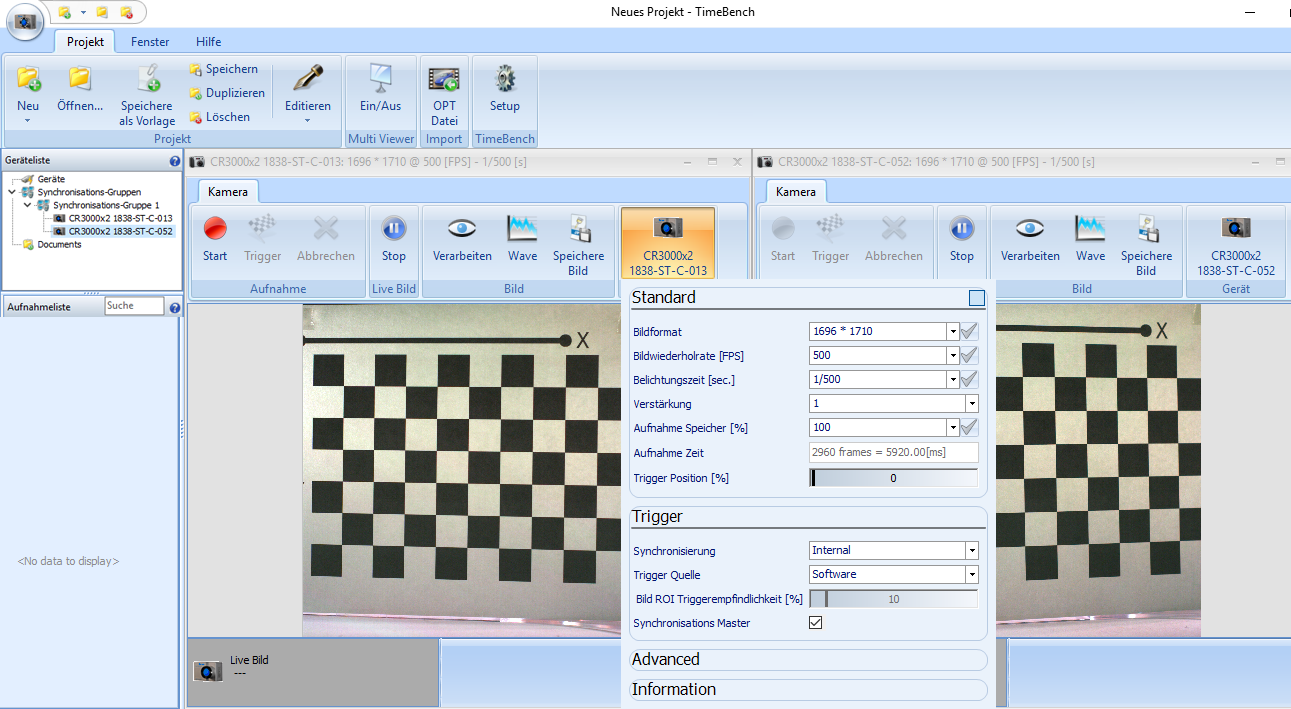
\includegraphics[width=1.0\textwidth]{figures/timebenchRecord}
		\caption[The views of two synchronized cameras and their capturing options in TimeBench]{The views of two synchronized cameras and their capturing options in TimeBench (\textit{source: software TimeBench owned by} \cite{Optronis.2016}).}
		\label{fig:timebanchRecord}
\end{figure}

Once the cameras are synchronized and configured the capturing of the calibration images can begin. The checkerboard pattern should be hold roughly at the same distance the objects will be placed in the actual scene. It needs to be in focus and must be fully visible in the view of both cameras. After starting the capturing sequence by clicking \enquote{Start} in the software and also activating the external trigger, the checkerboard pattern needs to be moved in different angles till the sequence stops. Out of the recorded image sequence 10-20 different image pairs have to be chosen (\autoref{fig:timebenchSequence} shows the timeline with the captured images of a session). Extreme angles are not likely to be detected later in MATLAB (\cite{StereoCalib.2016}).

\subsection{Estimating Stereo Parameters in Matlab}\label{ssec:estimateStereoParams}
The selected set of images pairs of the calibration pattern now need to be loaded into the Stereo Camera Calibration toolbox in MATLAB. They can be added by clicking \textbf{Add images} in the app. In the final experimental architecture the left camera is set as camera one and the right camera as camera two. In this step the correct size of the checkerboard squares are needed, in this case 3 mm. The images then get analyzed by the software, which can take a while depending on the amount and resolution of the set. The result window shows how many stereo pairs were added and how many were rejected, which can be displayed. The rejection can be cause of several reasons, which will be discussed and summarized in \autoref{sec:ExperimentalResults}. The data browser displays a list of all added image pairs, which should be checked whether they are sorted with their correct corresponding partners. Clicking on one pair of images the detected points are displayed in green color and can be checked more closely with the zoom function (\cite{StereoCalib.2016}).

After reviewing the accepted data, the button \textbf{Calibrate} will start the camera calibration. A diagram shows the overall \textbf{reprojection errors} in pixels\index{Reprojection error} from all images, which is the difference between the detected and the reprojected points, as shown in \autoref{fig:ReprojectionError}. The error should not be higher than 1 pixel but are recommended to be below 0.5 pixel. Outliers, which means errors much higher than the acceptable value, can be selected by moving the red horizontal line. The respective images can then be deleted in the data browser. After that \enquote{Calibrate} needs to be clicked again (\cite{StereoCalib.2016}).

\begin{figure}[htbp]
		\centering
		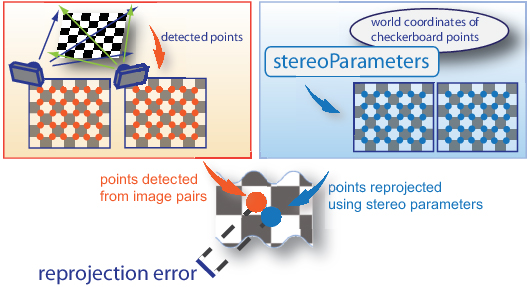
\includegraphics[width=0.9\textwidth]{figures/ReprojectionError}
		\caption[Calculation of the reprojection error]{Calculation of the reprojection error (\textit{source:} \cite{StereoCalib.2016}).}
		\label{fig:ReprojectionError}
\end{figure}

The bottom right window shows the estimated \textbf{extrinsic parameters}\index{Extrinsic camera parameters} in a \textit{camera-centric view}. If the pattern was stationary and the cameras were moved, the plot can be changed to a \textit{pattern-centric view}. This plot should be examined whether the relative poses of the cameras, the baseline and the checkerboard positions are matching the expected positions. 

Another factor to be reviewed is the \textit{rectification}. By clicking on \textbf{Show rectified} in the middle of the screen, the rectified image pair should be shown. If the rectified images are not undistorted and row-aligned the calibration was not accurate enough. This problem is further discussed in the session examples and in the summarized results (\autoref{sec:ExperimentalResults}).

\begin{figure}[htbp]
		\centering
		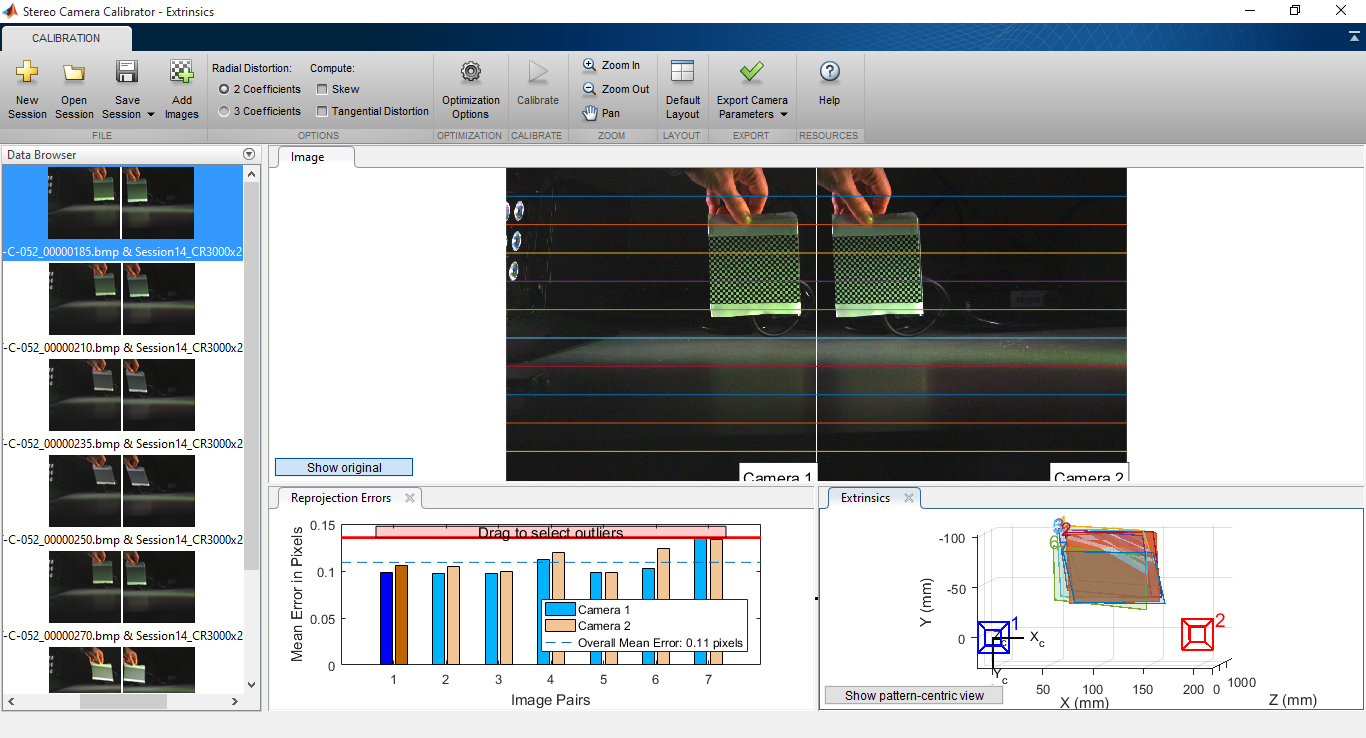
\includegraphics[width=1.0\textwidth]{figures/ExRectified}
		\caption[Calibrated camera system in Matlab]{Calibrated camera system in the Stereo Calibrator with: \textbf{(left)} data browser with set of accepted image pairs; \textbf{(middle)} rectified images of one image pair; \textbf{(bottom left)} reprojection errors; \textbf{(bottom right)} estimated extrinsic parameters.}
		\label{fig:ExRectified}
\end{figure}

The last step is to export the calibrated stereo camera parameters. \textbf{Export camera parameters} creates a \textit{stereoParameters object} in MATLAB's workspace and \textbf{Generate MATLAB script} saves the calibration steps of the session as well.

\subsection{The stereoParameters Object}\label{ssec:stereoParamsObj}
\todo{what does it mean}
\enquote{The object contains the intrinsic and extrinsic parameters of the camera, and the distortion coefficients. You can use this object for various computer vision tasks, such as image undistortion, measuring planar objects, and 3-D reconstruction}(\cite{StereoCalib.2016}).

\subsubsection{Calculation of the Fundamental Matrix}
\todo{do it!!!!!}			% Camera calibration
\section{Image Correction}

\index{Gaussian blur}
\begin{itemize}
\item Gaussian blur
\end{itemize}
\section{Image rectification}
\section{Point cloud}


\begin{itemize}
\item definition
\begin{itemize}
	\item \url{http://de.mathworks.com/help/vision/ref/reconstructscene.html#outputarg_pointCloud}
	\item \url{http://stackoverflow.com/questions/18994680/can-anyone-explain-the-difference-between-organized-and-unorganized-point-cloud}
	\item \url{http://pointclouds.org/documentation/tutorials/pcd_file_format.php}
	\item \cite{Rusu.2011} and \url{http://www.pointclouds.org/}
\end{itemize}
\item what can be done with pt clouds
\begin{itemize}
	\item refinement (see chapter refinement)
	\item stitch 3D point clouds together, 
	\item create surfaces from point clouds and visualize them
	\item extract keypoints and compute descriptors to recognize objects in the world based on their geometric appearance
\end{itemize}


\end{itemize}



%\input{triangulation}?
%\input{closure} 			% results/ interpretation ...
\section{Refinement}\label{sec:refinement}

\begin{itemize}
\item next to correcting the original input images, refining the output data set (the point cloud) to get out noise, but how?
\item different approaches and a test of each:
  \begin{itemize}
   \item mask (--> hardcoding --> bad!)
   \item Bundle Adjustment
   \item pcdenoise
   \end{itemize}
\end{itemize}

\subsection{Bundle adjustment}
see (\cite[p.320]{Szeliski.2011} and \cite[p.322]{Luhmann.2014})
and \url{http://grail.cs.washington.edu/projects/bal/}
Matlab provides a built-in method that refines camera poses and 3D points: the \textit{bundleAdjustment}\footnote{See a full description of the method at \url{mathworks.com/help/vision/ref/bundleadjustment.html}, 2016-05-03.}. In the following the bundle adjustment \index{Bundle adjustment} shall be used to refine 3D points so that reprojection errors get minimized. At this point it should be mentioned that the code for this method is rather sparsely documented, which could make the usage of the built-in method tedious. However, there are a lot more solutions to choose from provided by the community.

--> maybe use \url{https://github.com/tikroeger/BA_Matlab}
\todo{mathematical explanation what it is}

%\begin{lstlisting}

%\end{lstlisting}


\subsection{pcdenoise}
\todo{check real name of method}

\subsection{Pointcloud filters}
\url{http://docs.pointclouds.org/1.7.0/group__filters.html}
\begin{itemize}
\item filter outliers from noisy data (--> bundle adjustment), 
\item segment relevant parts of a scene, 
\end{itemize}

\subsection{Filter out distances}
- point cloud obj has x,y,z limits but they are read-only -.-
--> lets put custom box around it
- with the help of axis aligned bounding boxes (cite maybe gregory?)
- we only need 2 points for this, not min. 4 edges like in other bounding boxes
- we need 2 two points as vectors
- axis-aligned bounding boxes in (\cite[p.216]{Gregory.2014})
			% next steps
\section{Mesh Export}
	
\begin{itemize}
\item to be able to reuse and rework the 3d model one has to export the point cloud as a mesh/ surface
\item use pcwrite \footnote{The description of the method can be found at \url{http://mathworks.com/help/vision/ref/pcwrite.html}} to write 3d point cloud into PLY file
\item pcwrite(ptCloud,filename,'PLYFormat',format) 
	\begin{itemize}
	\item matlab function to write 3D point cloud to PLY file
	\item ptCloud: use output data
	\item filename: specify a filename
	\item PLY format: specified as the comma-separated pair consisting of the string format and the string 'ascii' or 'binary'. Use the binary format to save space when storing the point cloud file on disk.
	\end{itemize}


\item used software: meshlab \cite{Meshlab.2016}
\item MeshLab is an open source, portable, and extensible system for the processing and editing of unstructured 3D triangular meshes.
\item open source
\item amongst others it can import the following file formats: PLY, STL, OFF, OBJ, 3DS, COLLADA, PTX, V3D, PTS, APTS, XYZ, GTS, TRI, ASC, X3D, X3DV, VRML, ALN
\item meshlab example project need to be included, found in meshlab folder
\item Meshlabs measuring tool: measure objects to check sizes - gives the exact distance in units of the mesh --> or what units? not documented grrrrrrrr --> talk about problems with units in 3d
\end{itemize}


The tool was developed with the support of the 3D-CoForm project \footnote{The 3D-CoForm project aimed to establish a universal state-of-the-art in 3D-digitisation and 3D-documentation. The research reports and other information can be found at \url{http://www.3d-coform.eu/}.}

\begin{lstlisting}
pcwrite(ptCloud,'stillOwl','PLYFormat','binary');
\end{lstlisting}

\todo{The problem with units:} They are *all* measured in Units - no specific actual unit of measure, just raw 'units'... its then up to where you interpret that model as to how that program processes those units.

\url(http://animation.about.com/od/faqs/f/What-Are-Standard-Units-Of-Measurement-In-3d-Animation.htm)

That sort of explains it. You really need to think in just 'units' and NOT  a 'unit of measure' as it will trip you up in the future otherwise.

Anyway - Its a very important distinction - Units in 3D Space have *no* correlation to Inches or millimetres or any other 'unit of measure' - the file simply details the number of 'units'...

\todo{Points to Mesh}

\chapter{Closure} \label{c:Closure}			
\section{Closure}
\begin{itemize}
\item Problems encountered
	\begin{itemize}
	\item matlab (\autoref{ssec:Matlab})
	\end{itemize}
\item maybe use structure from motion (see also \cite{Gordon.2004})
	\begin{itemize}
	\item more views
	\item ideal for many pictures
	\item but will also take a lot of computational work
	\item and lighting!!!!
	\item relevant for many pt clouds: \url{http://www.mathworks.com/help/vision/examples/3-d-point-cloud-registration-and-stitching.html}
	\end{itemize}
\item what needs to be changed: cameras so they can be placed better next to each other, software...

\end{itemize}


\section{Future work}\label{sec:Future}
This will also include some suggestions on further readings.

\begin{itemize}
\item pt cloud refinement, stitching them together
\item object recognition
	\begin{itemize}
	\item describe what is possible (how), using this papers related research chapter: \cite{Lowe.2001} \url{http://www.cs.ubc.ca/~lowe/papers/cvpr01.pdf}
	\item and maybe this: \textit{Probabilistic Models of Appearance for 3-D Object Recognition}  \url{http://www.cs.ubc.ca/~lowe/papers/pope00.pdf}
	\item and maybe book: Digital image processin, ch. 12 --> in workshop
	\end{itemize}
\item --> robotic!!!
\item the void
\item hoodie \url{http://www.dezeen.com/2016/04/04/artefact-shadow-hoodie-virtual-reality-gaming-design-technology/}
\item microsoft hololens minecraft
	
\end{itemize}

\section{Acknowledgements}\label{sec:Ack}
-> sandra beuck grafik
-> alex sch. für technische beratung
-> betreuer for math. beratung
-> optronis technik zur verfügung stellen  
 			% fazit and future work
%\input{Acknowledgement} 	% evtl Danksagung???


\appendix
%\renewcommand{\indexname}{Stichwortverzeichnis} % Index umbenennen
\printindex					% Stichwortverzeichnis abbilden
\addcontentsline{toc}{chapter}{\indexname}
\listoffigures				% Abbildungsverzeichnis
%\listoftables				% Tabellenverzeichnis
%\lstlistoflistings			% Sourcecodeverzeichnis
\printbibliography[			% Literaturverzeichnis
	heading=bibintoc,
	title={Bibliography}]
% Literaturverzeichnis
	%\nocite{*} % muss später aufjedenfall raus
	%\bibliographystyle{alphadin} % for german type: alphadin
	%\bibliography{bibliography}
	
% to-do appendix:
% include checkerboard	
\end{document}